%\subsection{Screwdrive}
\label{sec:screwdrive}

%TODO: add screwdrive cover image

% Screwdrive locomotion subsection 
% Screwdrive images: https://docs.google.com/drawings/d/1YzuIb8U-4fQxipOJEBA4PD4eBe6fdJJcrUts8n2fkNc/edit 
%TODO: how does Dugoff define synthetic trafficability? 

%\subsubsection{Intro}

\begin{figure}[!htb]
	\begin{subfigure}[t]{0.5\textwidth}
		\centering
		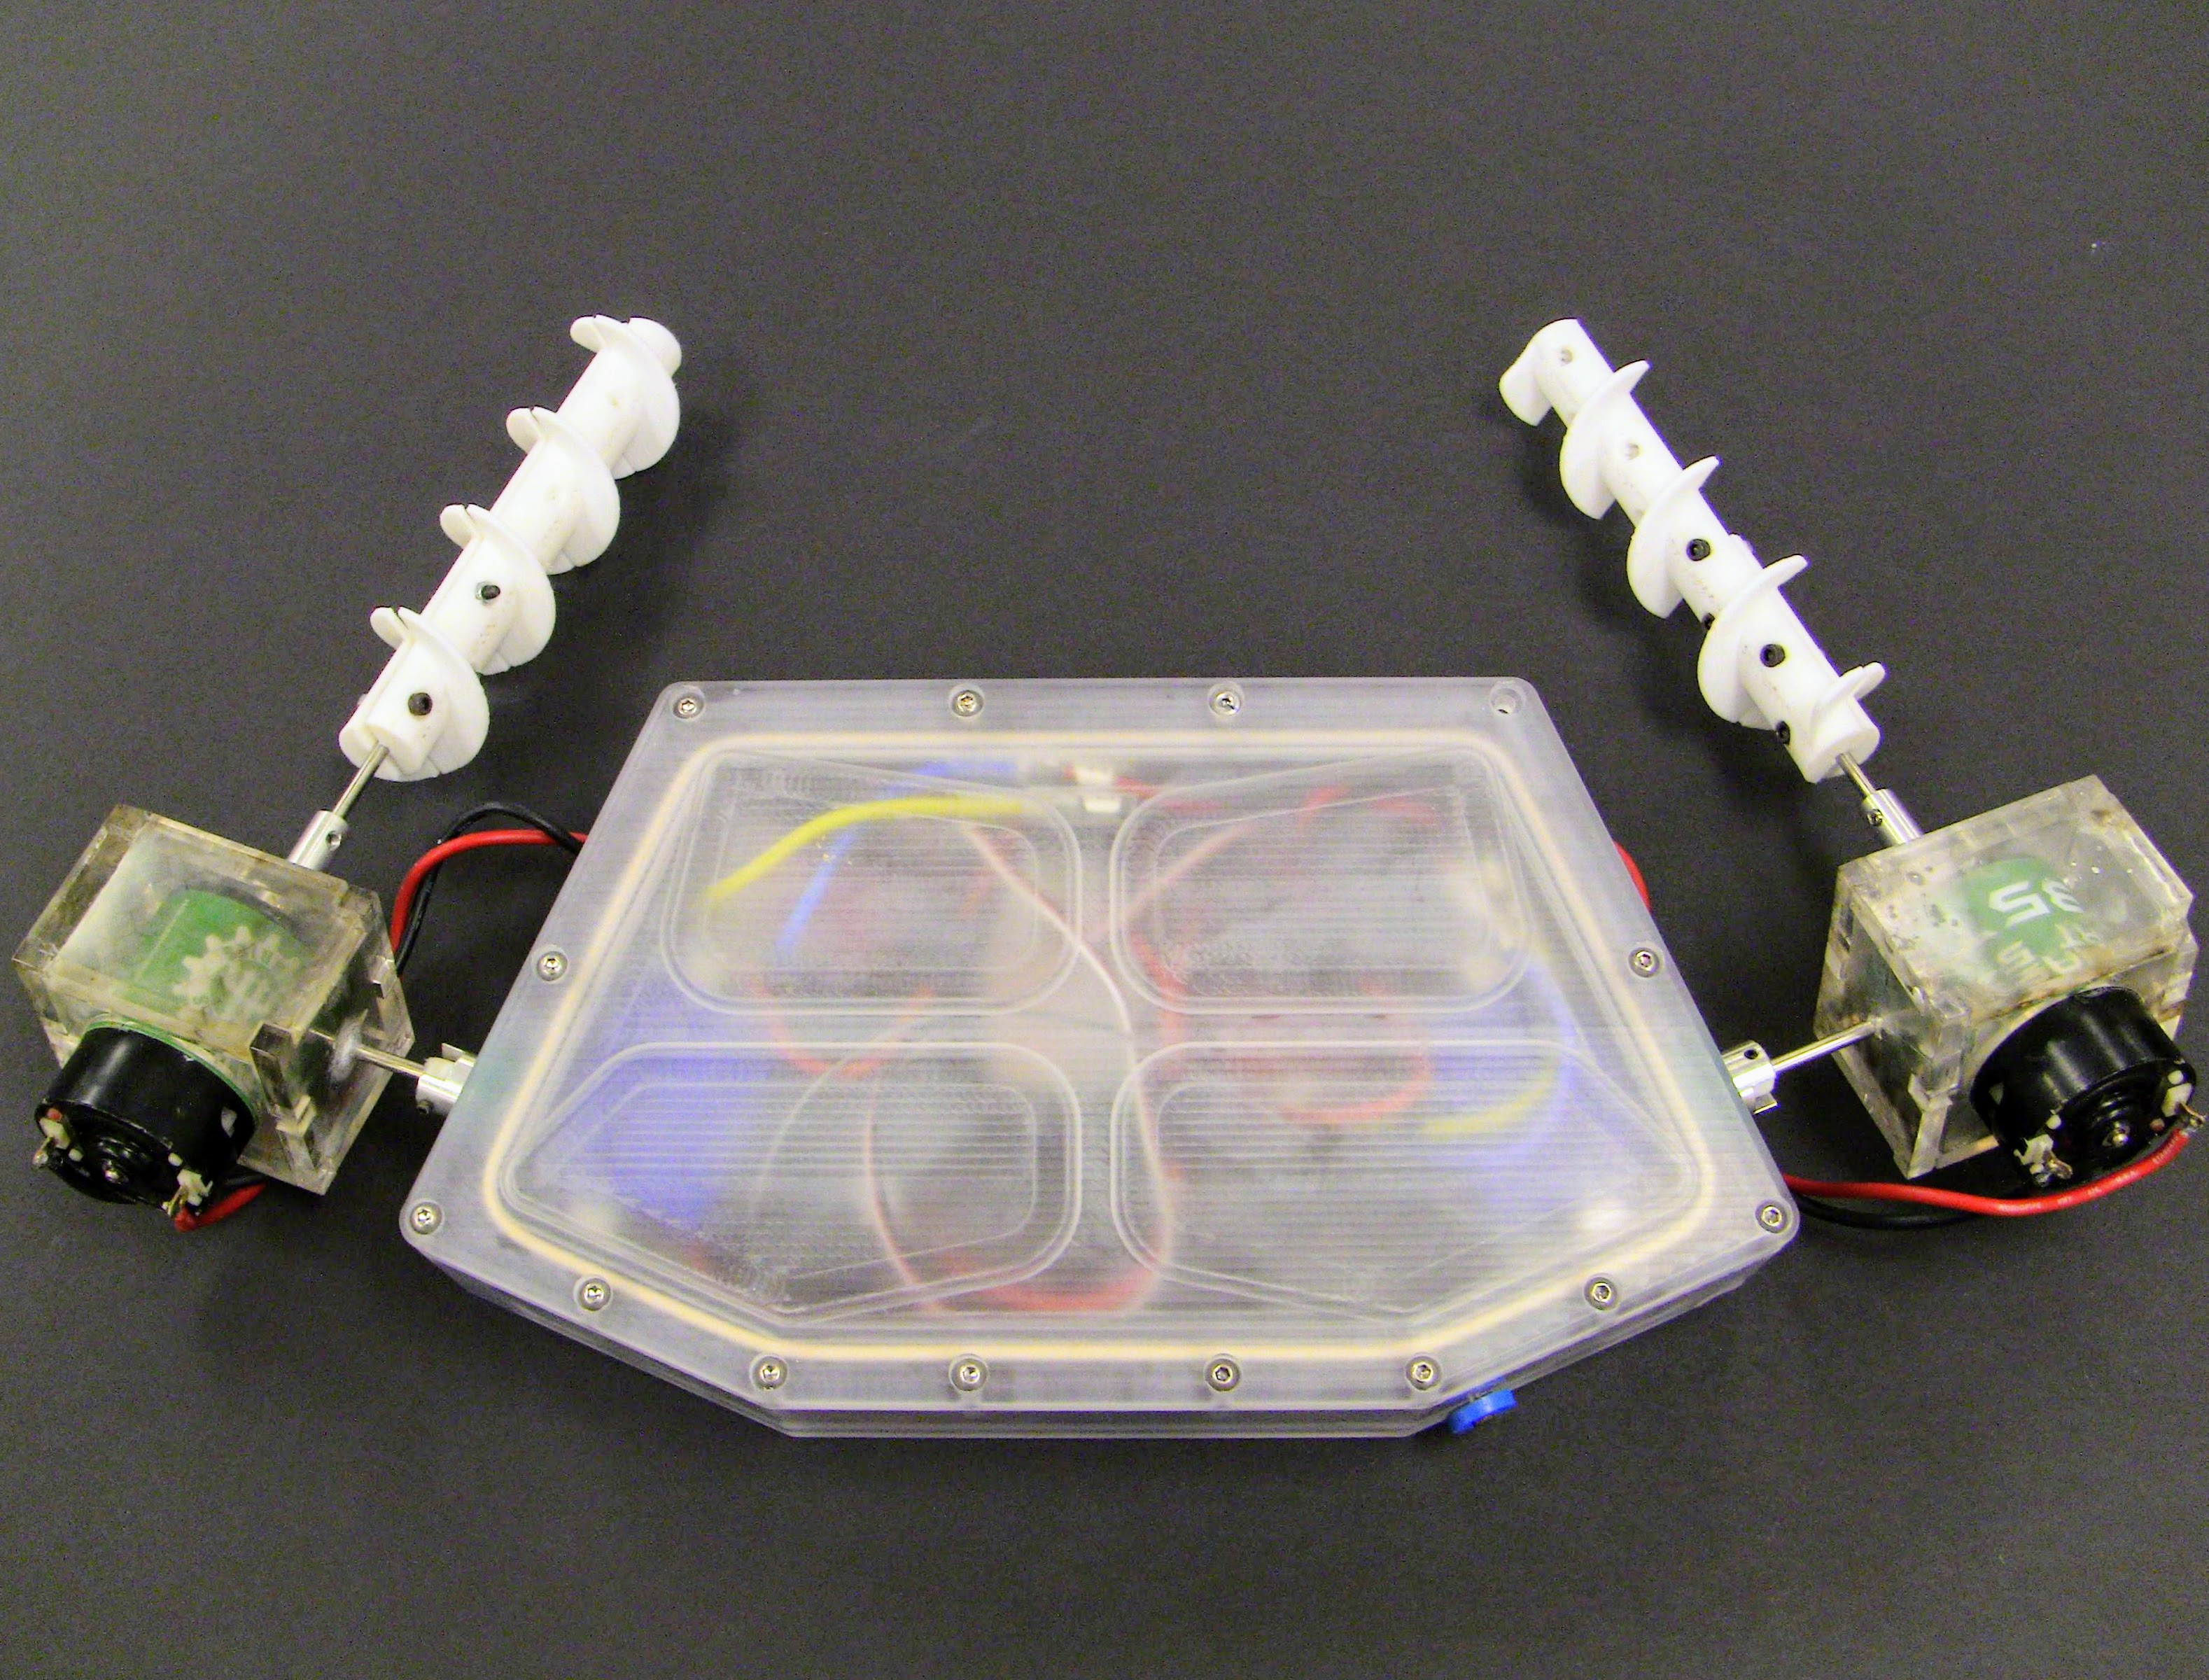
\includegraphics[width=\linewidth]{images/aquapod_v2_screwdrive.jpg}
		\caption{The dual screwdrive arms on the Aquapod v1}
		\label{fig:screwdrive_aquapod}
		%\vspace{-10pt}
	\end{subfigure}
	\begin{subfigure}[t]{0.5\textwidth}
		\centering
		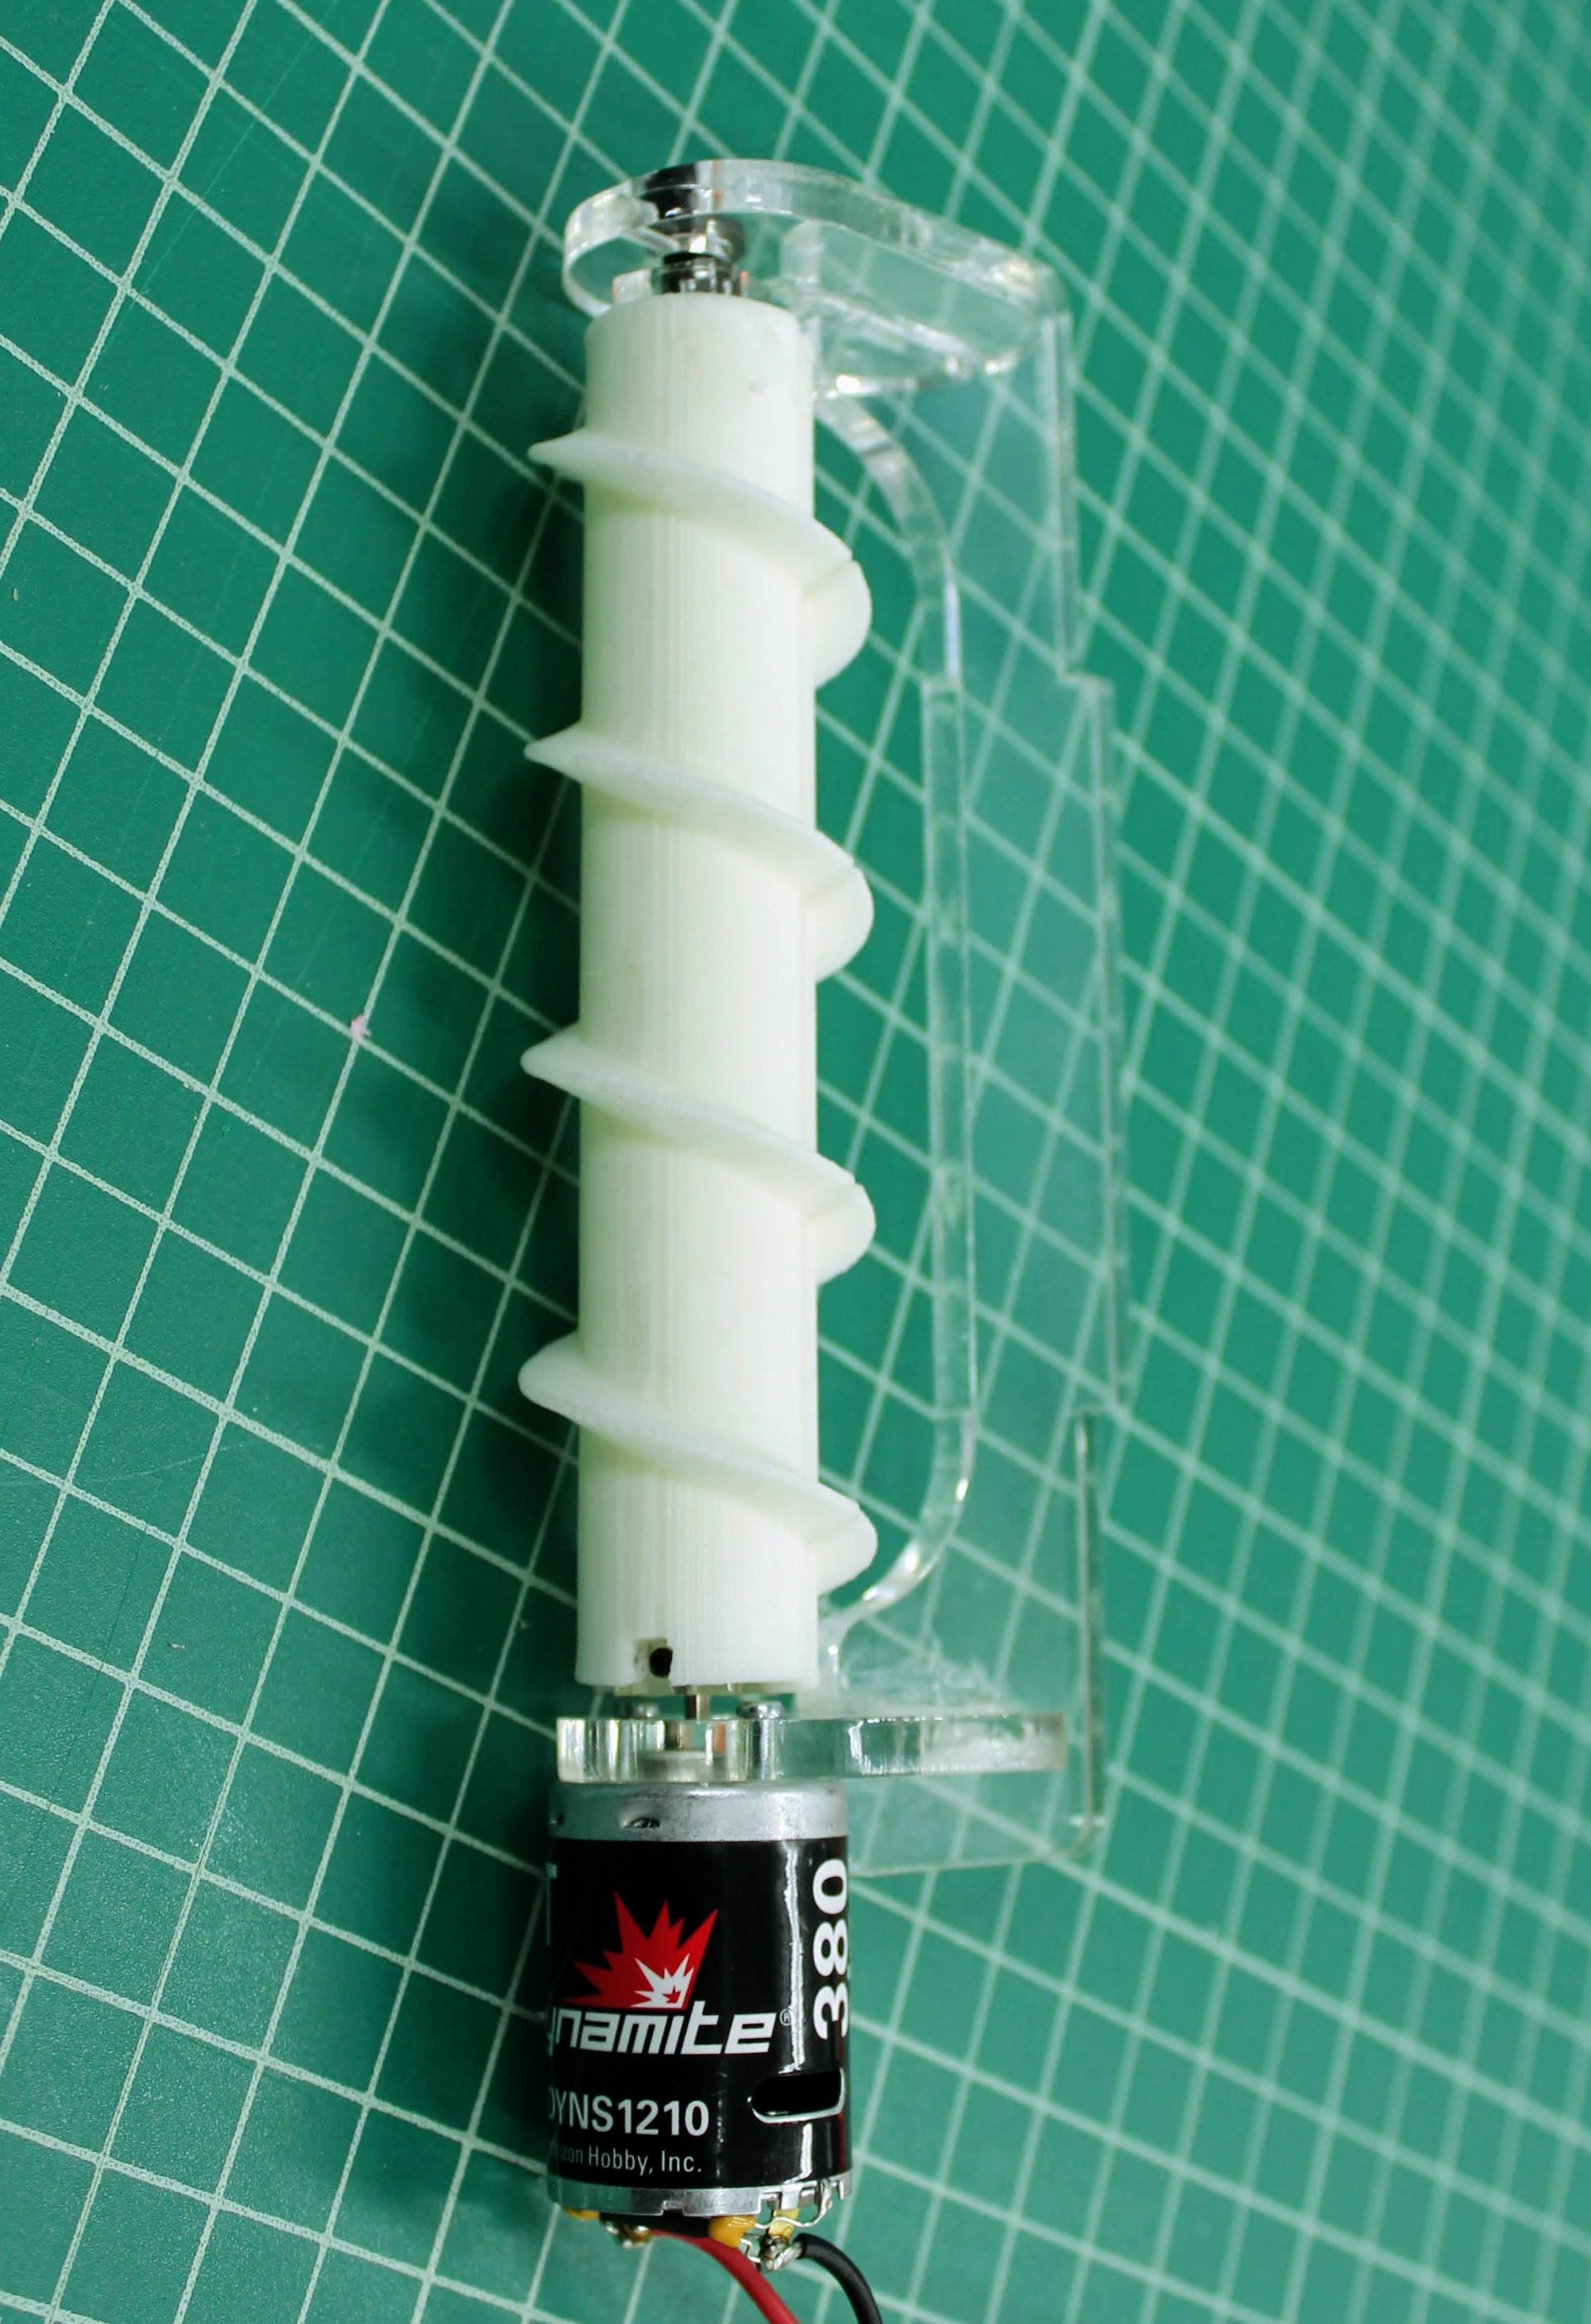
\includegraphics[width=0.5\columnwidth]{images/sd/screwdrive_omnibot_screw.JPG}
		\caption{Prototype screw}
		\label{fig:screwdrive_omnibot_screw} 
	\end{subfigure}
	\caption{Screwdrive screw prototypes}
	\label{fig:screwdrive_screw_prototypes}
\end{figure}

% why 
The motivation for research into amphibious modes of locomotion was born of two factors. One, to develop a suitable mode of locomotion for the amphibious Aquapod that could work on land, water, and terrains in between. Two, to complement tumbling locomotion with an alternative that would allow controllable steering. Steering would in turn permit motion planning as well as optimal obstacle approach for tumbling.

To complement tumbling and solve the controllability problem, the treaded Adelopod \cite{Hemes2011a} utilized a set of tank-like treads driven independently by DC motors to create a differential drive. This addition enabled predictable and more energy efficient motion control while using the original tumbling capability to overcome obstacles. Additionally, corner cases where the Adelopod could become stuck, due to legs or body jamming against the terrain, could now be overcome with the treaded drive in conjunction with arm actuation. 

%TODO: add treaded adelopod image

While treaded locomotion proved to be an inexpensive and simple solution to complement to tumbling on land, tread drives do not work well while completely submerged in water. Treaded drives have been used \cite{Kline2012} in amphibious applications albeit for surface vessels. Treads work in a manner similar to a paddleboat's wheel where propulsion is generated by the paddle pushing against water as it rotates. However, in a wheel, as with any cyclical system, as one paddle pushes in one direction, there is another paddle that provides propulsion of the same magnitude and opposite direction, resulting in no net propulsion. Treaded systems work when only partially submerged as one side of the treads pushes against water and the other against air, resulting in net propulsion.

In water, there exist many methods to provide actuation that range from the most simple flagellum-type propulsion mechanisms \cite{Regnier2014,Dhariwal2004, Edd2003}, to fish-like propulsion \cite{Yu2018,Massey1984}, and others such as anguilliform swimming \cite{Zhou2011}, however, with the exception of anguilliform locomotion, these methods do not work well or at all on land. %Could add bit about amphibious platforms here before diving into the DARPA amphibious vehicle. 

DARPA's most recent attempt into amphibious locomotion consists of a vehicle used in a logistics-enabling role, moving supplies from boats towards the shore. This vehicle, named the Captive Air Amphibious Transport (CAAT) \cite{Kline2012}, uses buoyant pontoons together with treads to move on the water's surface, then transitions to land and operates as a tank would. In the 1960s, the predecessor of DARPA, the Advance Research Projects Agency (ARPA) along with other government agencies funded research into another form of amphibious locomotion: \emph{the screwdrive}.

% screwdrive timeline
Screwdrive propulsion is a relatively neglected method of locomotion that has been shown to successfully propel military, scientific, and recreational vehicles across a wide variety of terrains ranging from snow to water and mud to sand \cite{Fales1972, Cole1961, Dugoff1967}. This method of locomotion can trace its roots back to 1804 when Colonol John Stevens took the Archimedes screw concept and applied it to drive a steamboat on New York's North River \cite{Dugoff1967}. Screws then found use in land-based applications in the form of the Fordson tractor \cite{Freeberg2010} in the 1920s. There was a proposal in 1948 for a screw-propelled amphibious vehicle in England \cite{Cole1961}. Additionally in 1957 a German firm also demonstrated a screw-propelled amphibious vehicle during the Hanover Exhibition. The USSR found use for screw-driven vehicles to retrieve space cosmonauts from terrains consisting of deep snow \cite{Freeberg2010}. 

% research timeline
Most of the available research into screwdrive locomotion and its design parameters dates back to the 1960s and 1970s when Dr. Cole \cite{Cole1961}, of the University of Birmingham in England, and the Chrysler Defense Corporation \cite{Fales1972, Dugoff1967}, through US Military funding, carried out research in this method of locomotion for littoral environments. Recently, Freeberg et at. \cite{Freeberg2010} conducted research on quad-screw configuations and compared its performance relative to the traditional dual-screw. Nagaoka et al. \cite{Nagaoka2011} have explored the modeling of a dual screw system in compliant terrain, specifically moon soil, or regolith. Both Freeberg and Nagaoka studied the peculiar maneuverability charecteristics of screwdrive systems as these are relatively unexplored compared to traditional locomotion methods. In the field of robotics, screwdrive propulsion is not common, however, it presents a mechanically-simple, robust, inexpensive, and multi-domain method of locomotion. 

% TODO: update to reflect current structure 
The following section will focus on the parameters that define functional characteristics of screwdrives. The next section covers the particular maneuverability properties of screwdrive systems. Finally, proposed research on screwdrive systems is covered in the last section. 


%\subsubsection{commented out text }
%The U.S. military started research on the screwdrive by retrofitting a Weasel tank with screws. Formal research on the parameters of screw propulsion didn't start until the 1960s with Chrysler Defense Corporation \cite{Dugoff1967} \cite{Kress1965} and Dr. B.N. Cole in England \cite{Cole1961}. These two research initiatives form the bulk of known research into this form of locomotion. That being said, screwdrive locomotion has been used for mining applications such as the Mudmaster, the Snowbird platforms which were used in attempts and ultimate success crossing the Bering Strait, the Spiral Track Autonomous Robot of Lawrence Livermore National Laboratory \cite{Perez1996}, and the Tyco Terrain Twister toy remote controlled vehicle.

%The above mentioned applications had various things in common. Terrains that were found to be best for screw-propelled locomotion, herein referred to as screwdrive locomotion, were terrains that were marshy, snowy, or icy. Much like the Aquapod, for exclusively moving on water or land domains, there are better ways locomote. Another commonality is that, excluding the Terrain Twister, all vehicles above employed dual parallel screws for lomotion. A notable exception is the Terrain Twister that uses an additional actuator to alter the angle between the screws, similar to the Adelopod \cite{Hemes2011}. Freeberg \cite{Freeberg2010} explored and compared different screw configurations against the conventional dual screw design. 

%An important characteristic of screwdrive locomotion is that it is highly dependent on the terrain in which it operates, as described in \cite{Cole1961}, \cite{Kress1965}, \cite{Dugoff1967}. This presents both an opportunity and a challenge. It's a challenge in the vehicle model will necessarily then depend on the terrain, this is because the screw blade must be able to cut into the medium in order to create forward travel \cite{Freeberg2010}. Dual systems are typically oriented parallel to the longitudinal axis of the body, and if the blade is not able to penetrate the ground, then the screws essentially turn into rollers, in which case only lateral motion is possible. 

%In water, this is not an issue, since the screw acts like one long continuous blade. In snow and certain kinds of mud, screwdrives have been found to work exceptionally well, not only providing adequate locomotion, but exceeding what other modes are capable of \cite{Gorton1963}. Neumeyer et al \cite{Gorton1965} provided extensive mobility tests with the Marsh Screw Amphibian (MSA) in water, sand, mud, and snow, among other terrains. Additionally, screwdrives have been found to work well on ice, again, however, this is dependent on the blade's ability to penetrate the ground. This in turn is affected by factors such as blade thickness, blade height, and weight carried by the blade as well as a number of the terrain's properties such as compaction, moisture content, soil strength, among others \cite{Knight1965}, \cite{Dugoff1967}. 



%-------------------------------------------------------------------------------------------------------
\subsubsection{Screwdrive Design Parameters}
\label{sec:screwdrive_parameters}
%-------------------------------------------------------------------------------------------------------

% screwdrive params. and maneuver.
\begin{figure}[htb]
	\begin{subfigure}[t]{0.5\textwidth}
		\centering
		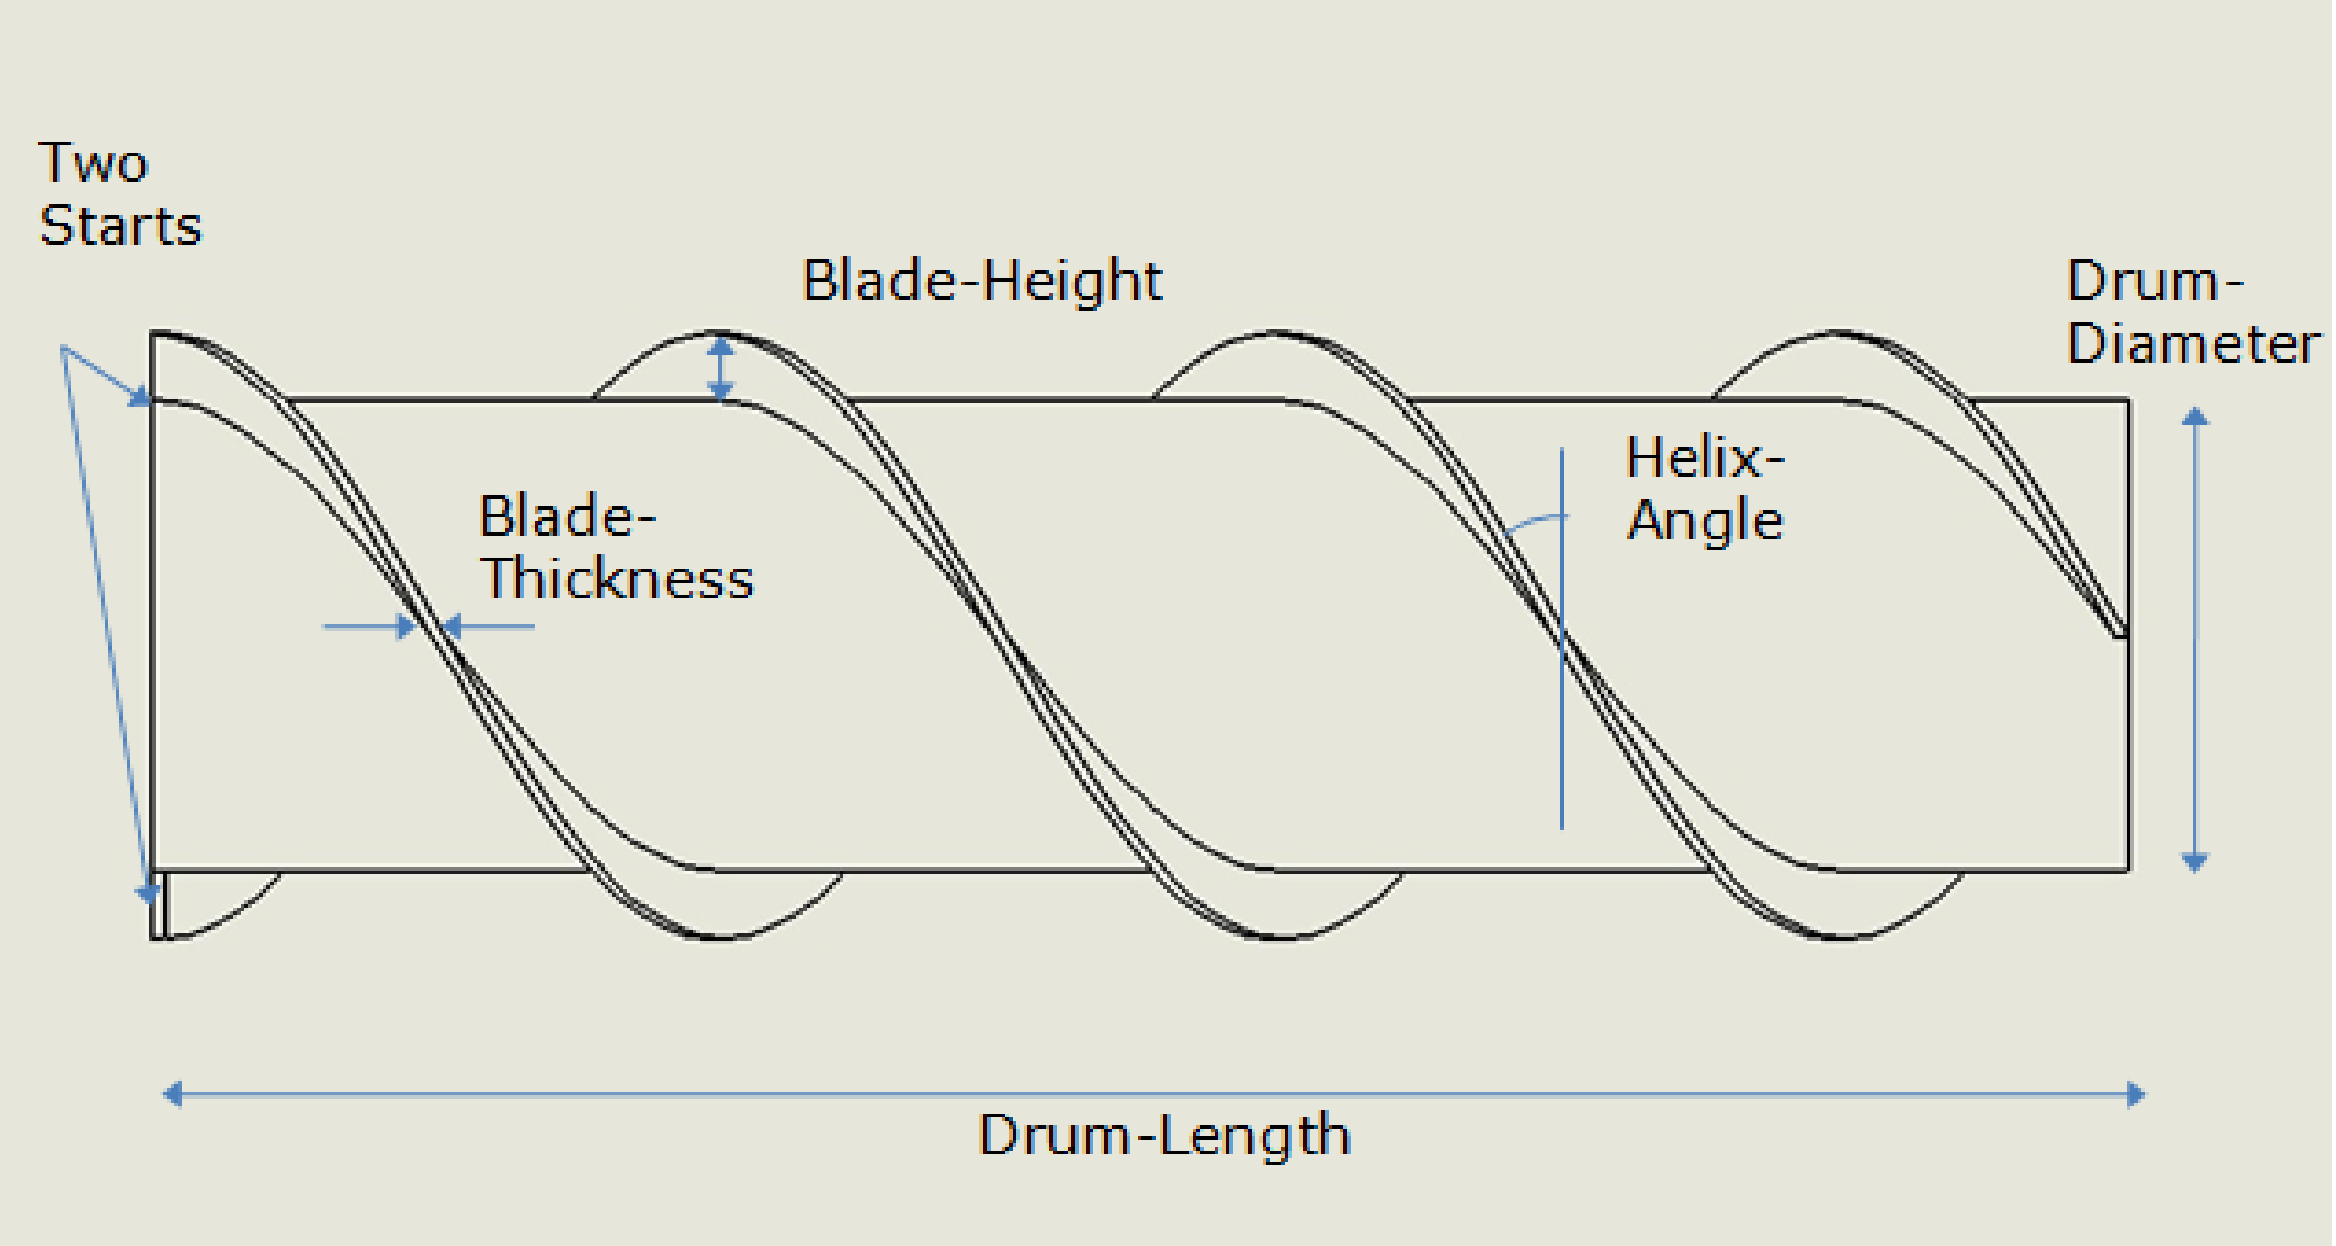
\includegraphics[width=1\columnwidth]{images/sd/screwdrive_parameters_freeberg.png}
		\vspace{-10pt}
		\caption{Screw Design Parameters \cite{Freeberg2010}}
		%\vspace{-20pt}
		\label{fig:screwdrive_parameters}
	\end{subfigure}
	\begin{subfigure}[t]{0.5\textwidth}
		\centering
		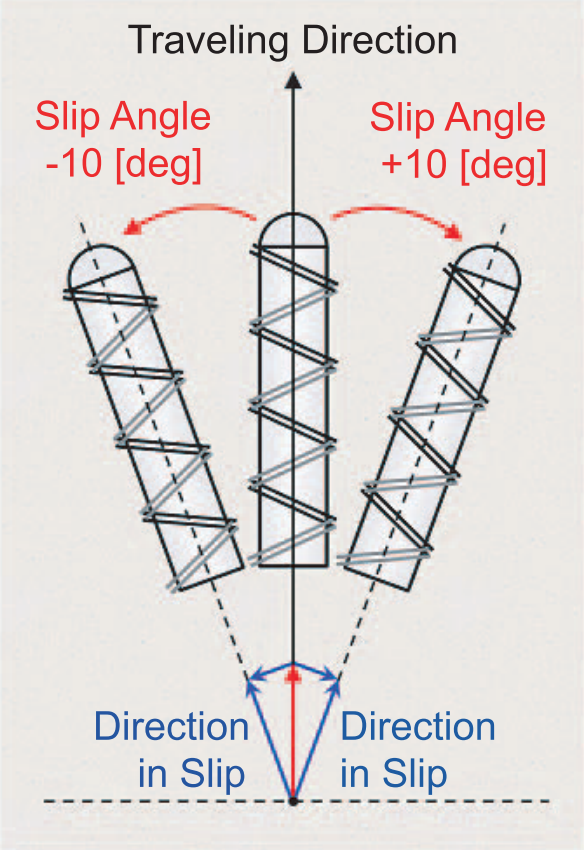
\includegraphics[width=0.5\columnwidth]{images/sd/screwdrive_slip_angle_nagaoka.PNG}
		\caption{Slip angle \cite{Nagaoka2011}}
		\label{fig:screwdrive_slip_angle} 
	\end{subfigure}
	\caption{Screwdrive characteristics}
	\label{fig:screwdrive_characteristics}
\end{figure}



%%screwdrive on aquapod
%\begin{figure}
  %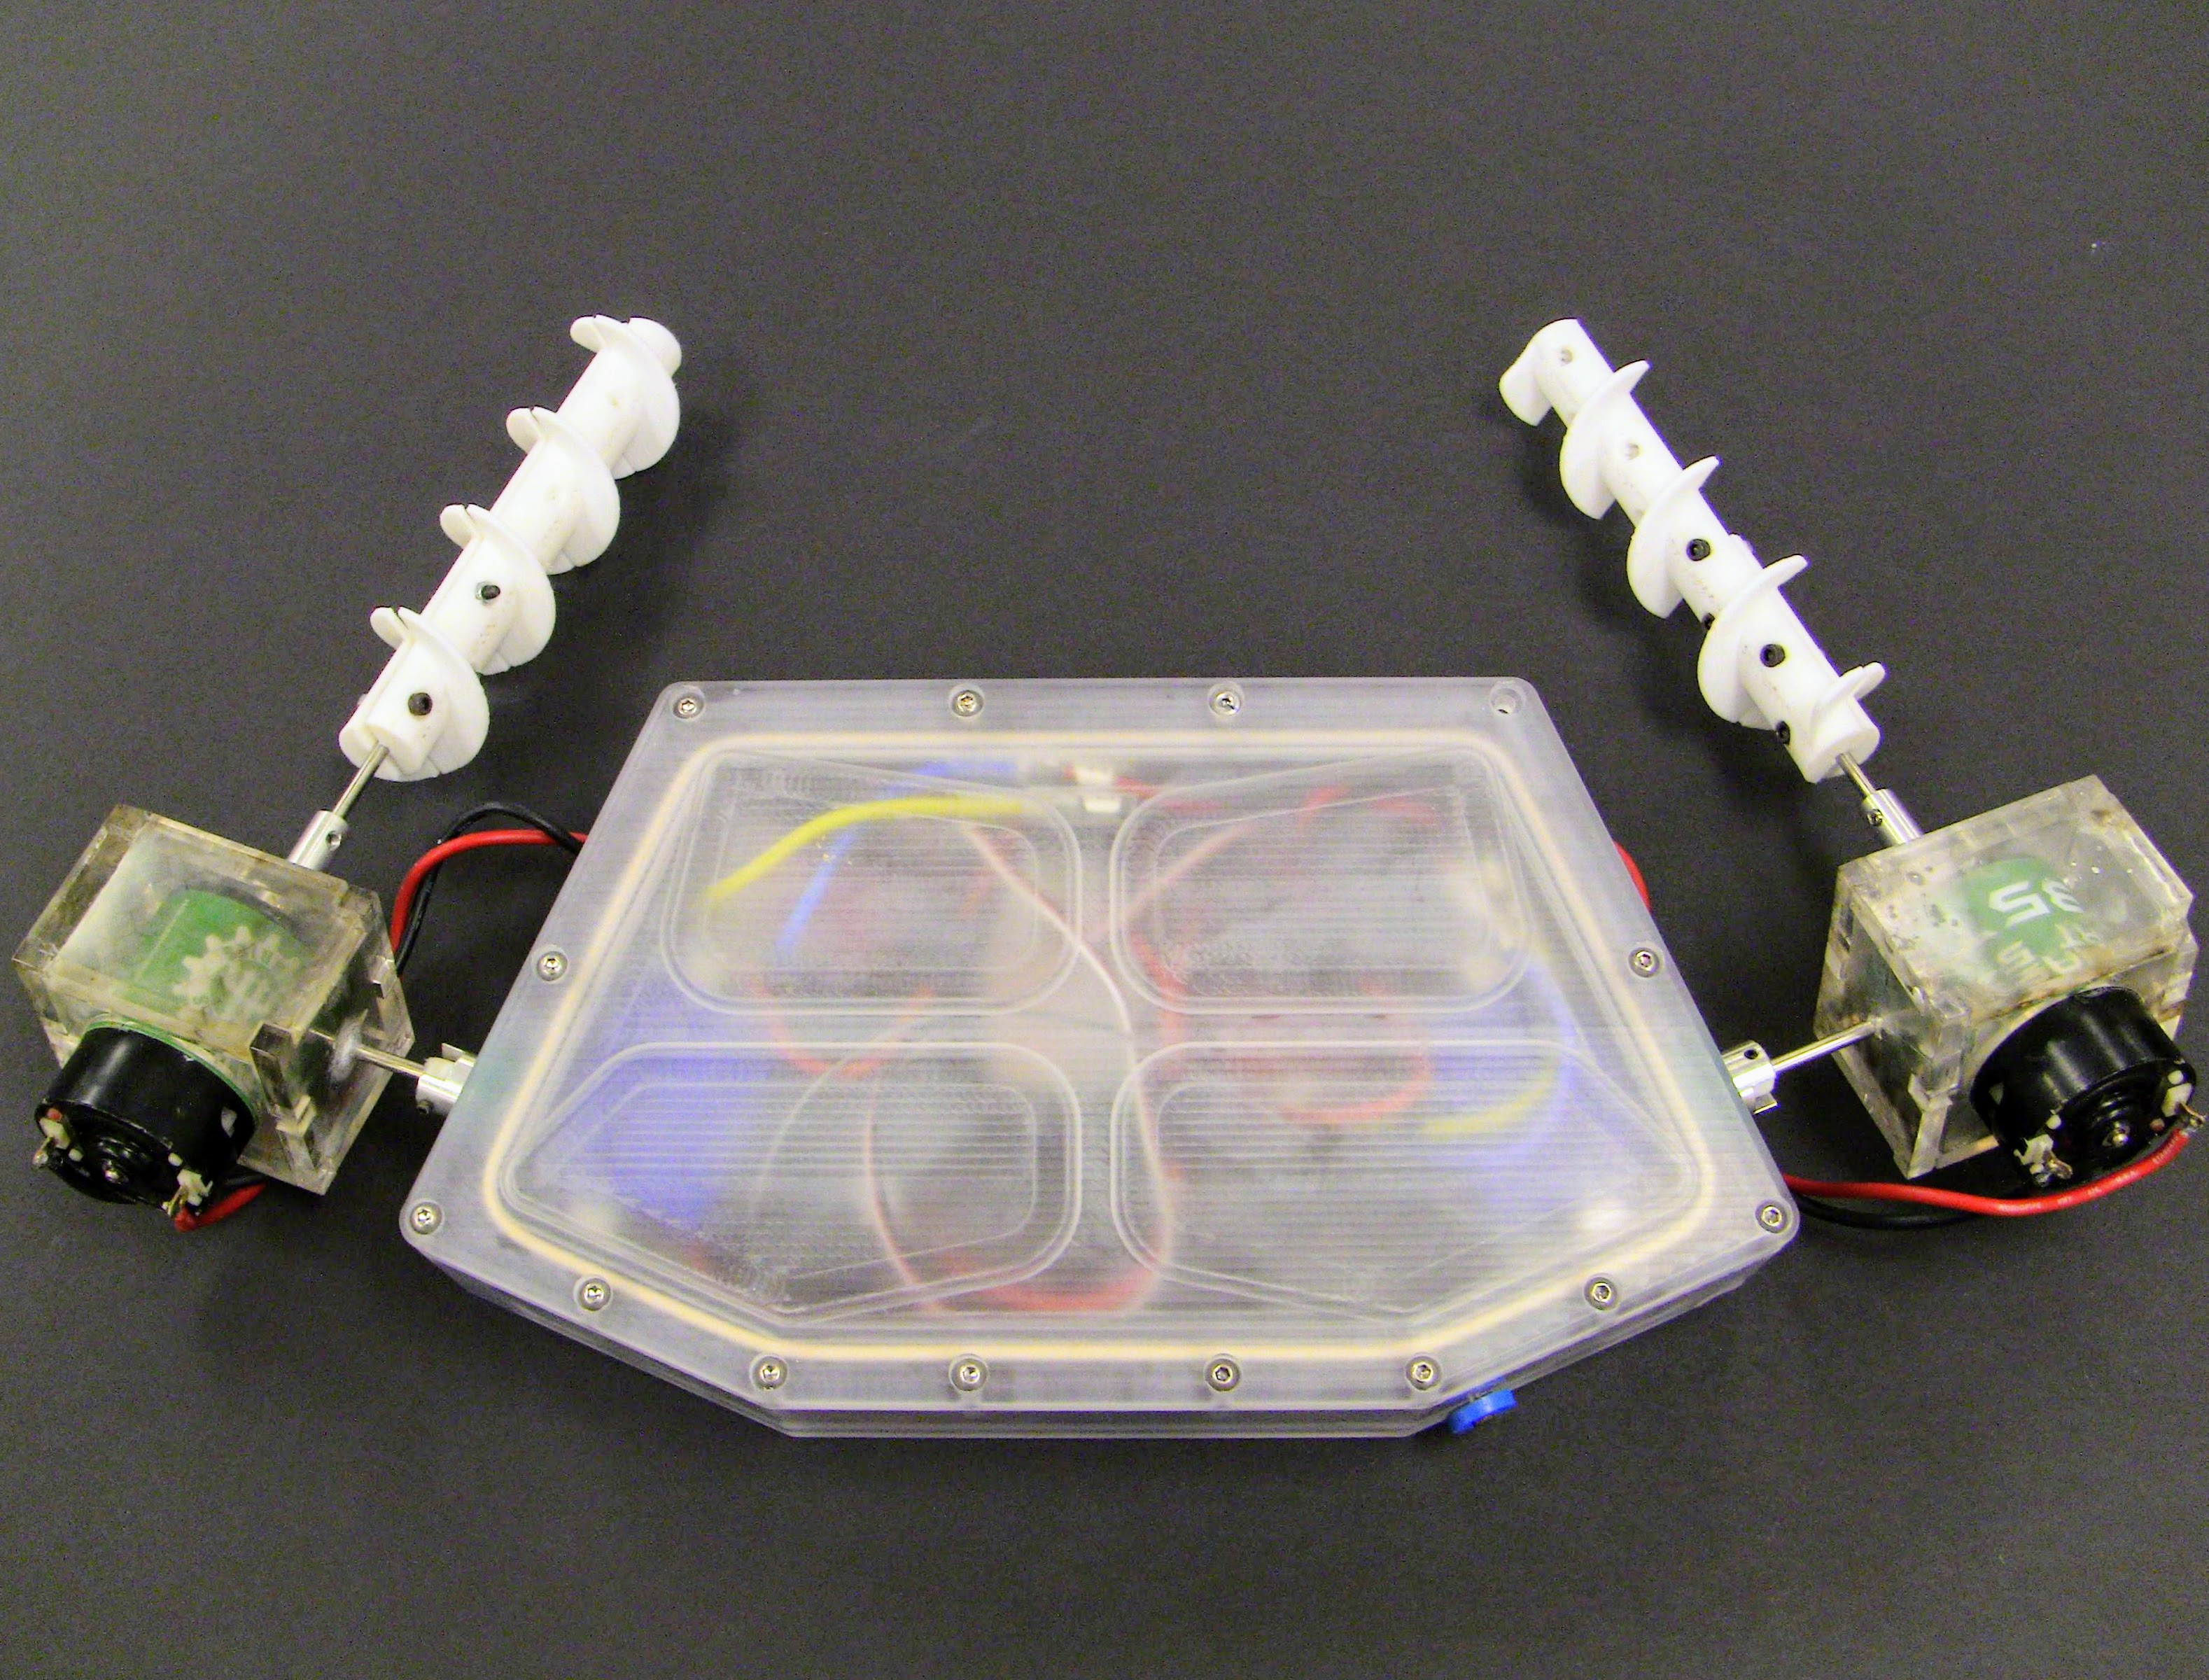
\includegraphics[width=\linewidth]{images/aquapod_v2_screwdrive.JPG}
  %\caption{The dual screwdrive arms on the Aquapod v1}
  %\label{fig:screwdrive_aquapod}
%\end{figure}



A screwdrive system is one that uses the rotation of one or more screws to generate motion. The majority of research in this area has focused on parallel dual-screw systems which consist of two contra-rotating screws are placed on either side of the vehicle body as a substitute for wheels or tank-treads. The Riverine Utility Craft and Dr. Cole's prototype, as seen on figure \ref{fig:screwdrive_prototypes}, are examples of dual-screw systems. 

%Figure~\ref{fig:screwdrive_aquapod} shows a dual-screw configuration in which the screws form an angle with respect to one another, this is called the \textbf{\emph{inter-screw angle}}. The inter-screw angle is important because it affects the resulting force balance between the screws, thereby affecting motion. 

The screw itself is comprised of two main parts: a barrel body and a blade that winds itself in a helical shape around the barrel body, as shown in Figure \ref{fig:screwdrive_parameters}. The barrel serves for mechanical support, and in some cases buoyancy, while the blade is the element that provides longitudinal locomotion. As the screw rotates, the blade travels longitudinally interacting with the medium against the blade. In the case of water, the displacement of the fluid provides thrust. In the case of a penetrable terrain, it is the combination of displacent and burrowing that provides the motion. In the case where there is no penetration of the medium by the blade, there would be no longitudinal component and rotation of the screw would be no different than rotation of a roller or wheel. 



The angle, \emph{\( \alpha \)}, that the blade makes with respect to the longitudinal axis of the screw is called the \emph{helix angle} or \emph{pitch angle}. The \emph{pitch angle} is one of the most influential parameters of a screw, as it determines the relationship between the rotational velocity and forward advance speed of the screw. The greater the \emph{helix angle}, the greater the rate of advancement. 

%TODO: COULD add image of screw with different pitches

%The screw blade is wound in a helix around the barrel body, as the screw rotates, the medium against the screw blade is pushed along the axis of the screw resulting in a longitudinal motion. In the case where there is no penetration, there would be no longitudinal component and rotation of the screw would be no different than rotation of a roller or wheel. 

The height, \emph{h}, of the blade is also an important parameter, as is the ratio of the blade height to the barrel diameter, this is referred to as \emph{blade-height-to-drum-diameter-ratio}. These parameters affect the amount of material the blade interacts with, which then influences thrust generated, torque requirements, drawbar-pull, among others. In a similar way, the number of starts the blade has, \emph{N}, is also important in controlling the amount of screw blade surface area in contact with the medium. Another geometric parameter of importance is the \emph{screw length}, this has also been expressed in terms of the \emph{length-to-drum-diameter-ratio} in studies. 

%The design of the screw itself is simple and enclosed, leading to robustness to mechanical failure and clogging when compared with other methods of locomotion\cite{Nagaoka2009b}. Screwdrives can function even when fully buried, this is advantageous in a number of situations such as snow, loose sand, mud, etc. 

The majority of the research into screw drive design and its parameters was conducted by Dr. Cole \cite{Cole1961} and Chrysler Defense Corporation \cite{Dugoff1967, Knight1965, Fales1972, Gorton1965} and utilized the parallel dual-screw configuration. On these screws, the helices were wound about the barrel in opposite handedness. Dr. Cole built  scaled-down prototype seen in Figure ~\ref{fig:screwdrive_cole_model}, while Chrysler built 1/8 and 1/5 scale prototypes, to carry out parameter optimization and trials, before building the full scale Marsh Screw Amphibian (MSA) and the later Riverine Utility Craft (RUC), \ref{fig:screwdrive_ruc}.

%TODO: add Cole and Chrysler prototype images 
\begin{figure}[tb]
	\begin{subfigure}[t]{0.5\textwidth}
		\centering
		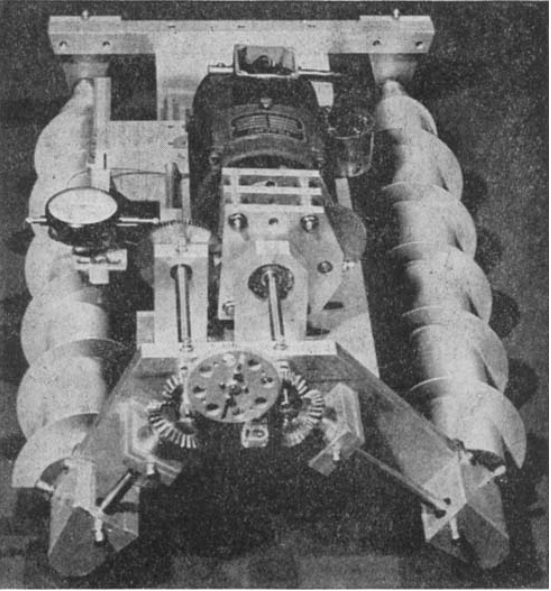
\includegraphics[width=1\columnwidth]{images/sd/screwdrive_cole_model.PNG}
		\vspace{-10pt}
		\caption{Dr. Cole's prototype model \cite{Freeberg2010}}
		%\vspace{-20pt}
		\label{fig:screwdrive_cole_model}
	\end{subfigure}
	\begin{subfigure}[t]{0.5\textwidth}
		\centering
		%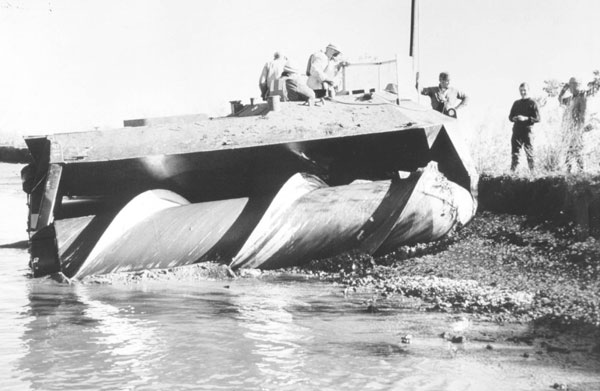
\includegraphics[width=1\columnwidth]{images/sd/screwdrive_ruc.PNG}
		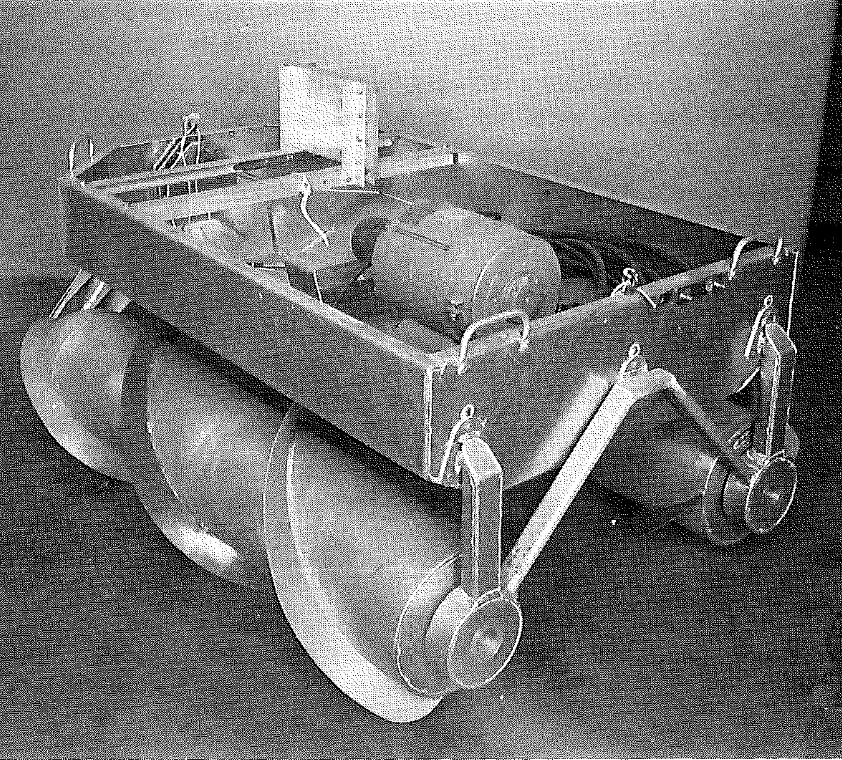
\includegraphics[width=1\columnwidth]{images/sd/screwdrive_ruc_fales.PNG}
		\caption{Riverine Utility Craft \cite{Fales1972}}
		\label{fig:screwdrive_ruc} 
	\end{subfigure}
	\caption{Screwdrive prototypes}
	\label{fig:screwdrive_prototypes}
\end{figure}

% other prototypes: http://www.oobject.com/category/9-screw-drivers/ 


Prototypes of various scales were built to evaluate and determine the optimal screw design parameters for water, ground, and  everything in between such as mud, snow, sand, and other terrains. The Marsh Screw Amphibian was tested in the Detroit River for more than 100 hours. 124 trafficability tests were performed in Louisiana by the US Army Engineer Waterways Experiment Station while a secondary MSA was built and tested for snow conditions in Houghton, Michigan \cite{Gorton1965}. 

Dr. Cole studied both screwdrive locomotion both aground and afloat. On ground, Cole \cite{Cole1961} found that vehicle performance gap, a measure of efficiency parameterized by screw slippage and power consumption, was less in the \emph{pitch-angle} range of 30 to 40 degrees than 20 to 30 degrees.  Drawbar-pull was almost maximum at 30 degrees, with little improvement with increasing helix angle. Therefore, from Cole et al. \cite{Cole1961} and Chrysler \cite{Dugoff1967, Fales1972} a value of 30 degrees or slightly greater was optimal. The Riverine Utility Craft \cite{Fales1972}, which was a continuation of the Marsh Screw Amphibian \cite{Dugoff1967}, utilized a pitch angle of 32 degrees.

With respect to \emph{blade-height-to-drum-diameter-ratio}, Cole used 0.375 as the ratio in his experiments finding it a sufficient tradeoff between propulsive surface area and structural integrity of the blades. Dugoff et al. \cite{Dugoff1967} utilized ratios of 0.125, 0.167, and 0.208 and found that increasing the height also increased the amount of media moved, however, its effect on drawbar-pull was minimal in sand. On mud, an increase in height resulted in decreasing performance due to greater likelihood of bogging down. Eventually 0.125 was chosen as an ideal ratio.

Another important parameter is the \emph{number of starts}, while Chrysler does not make available data on the number of starts, both the MSA and the RUC \cite{Knight1965} used two screw starts, with Dr. Cole making the case that two starts may grant better dynamic balancing. 

Unlike the monotonic effects of the \emph{helix angle} and \emph{screw blade height} on the drawbar-pull capacity, the \textbf{\emph{length-to-drum-diameter-ratio}} was found to follow a concave curve. These studies were carried out for mud and sand and, coincidentally, the optimal value for both terrains occurred at around 6. In water, Dr. Cole found that longer screws led to more rotations and consequently larger driving torques and thrust.  

Although important in terms of design and manufacture, \emph{blade thickness} was not studied explicitly. It was noted that during operation, the Riverine Utility Craft screws began to develop cracks along the blade. The cause of the cracks was thought to be from forces on the screw blade, given that the screws had passed preliminary shock tests. The solution was to this problem was to add structural reinforcement to the back of the screw blade. 

Not a parameter of the screw itself, the \emph{center-of-gravity} affects the pitch of the vehicle, leading to bulldozing or plowing if located too far forward and suboptimal performance if placed too far towards the rear \cite{Dugoff1967, Nagaoka2011}. 

The \emph{slip angle} is another parameter that is not of the screw but affects the function of the vehicle. Experiments on a custom rig showed that drawbar pull increased significantly when the slip angle, which is the angle of the screw relative to motion of the vehicle, was deviated from parallel for a variety of speeds. Furthermore, the drawbar pull displayed increased for positive angles, but decreased with negative slip angle. This would suggest that the more perpendicular the screw blade is relative to vehicle motion, the larger the drawbar pull. This would also correlate other experiments from Nagaoka \cite{Cole1961} that measured drawbar-pull against \emph{helix angle}. If this is the case, one could alter the screws' \textbf{\emph{helix angle}} to compensate for screws that are oriented at an arbitrary \textbf{\emph{slip angle}} with respect to the vehicle's body, such as the Aquapod as seen in Figure ~\ref{fig:screwdrive_aquapod}, to obtain optimal performance.

Clearly, the parameters of the screws affect a screwdrive system's performance on a given terrain, while Dugoff et al. \cite{Dugoff1967} utilized parameters that balanced the performance on water and on land, there exist parameter configurations that maximize screw performance in other domains. Furthermore, while Cole \cite{Cole1961} and Dugoff \cite{Dugoff1967} both studied screw parameters, blade penetration of the terrain was greatly facilitated by the relatively heavy weight of the tank-sized vehicles. Additionally, while drawbar pull, or towing capacity, was an important outcome metric for the aforementioned applications, at the smaller and lighter scale of environmental robotics, parameters to increase mobility would be more relevant. 

In the next section the maneuverability of screwdriven vehicles is explored. 

%The parameters mentioned affect the ability and the way that a screwdrive propelled vehicle moves throughout an environment. In the next section the maneuverability of screwdriven vehicles is explored. 

%Nagaoka \cite{Nagaoka2011} and Cole \cite{Cole1961} showed that forward speed was proportional to rotational speed, therefore indicating constant slip conditions. % #parameters %TODO: check on Cole/Dugoff reference for forward-speed to rotational velocity relation independence on other factors. 

	%\emph{Inter-screw angle:} the inter-screw angle is the angle between two or more screws. This angle playes a pivotal role as it affects the interplay of forces and resulting motion of a vehicle. In systems with two independently actuated screws, the inter-screw angle affects the resulting motions from the net forces of the competing or cooperating screws. The redirection and interplay of the forces from the dual-screw set-up can be seen in Figure~\ref{fig:screw_FBD_alpha_0} and Figure~\ref{fig:screw_FBD_alpha_45} where the inter-screw angle is set to 0 and 45 degrees, respectively. Figure~\ref{fig:screw_FBD_alpha_0} shows the direction of the force when the blade is engaged. This mode is optimal for a screwdrive system because the direction of the force together with the independence of the actuators can be used to move the vehicle forward, backward, laterally, and to allow rotations in place, in effect, omnidirectional locomotion. 





%\begin{figure}[ht]
%	\centering
%	\includegraphics[scale=0.25]{images/screw_propulsion_FBD_alpha_0.pdf}
%    \caption{Inter-screw angle of 0 degrees (parallel)}
%	\label{fig:screw_FBD_alpha_0} 
%\end{figure}
%\begin{figure}[th]
%	\centering
%	\includegraphics[scale=0.25]{images/screw_propulsion_FBD_alpha_45.pdf}
%    \caption{Inter-screw angle of 45 degrees}
%	\label{fig:screw_FBD_alpha_45} 
%\end{figure}

%-------------------------------------------------------------------------------------------------------
\subsubsection{Maneuverability}
\label{sec:screwdrive_maneuverability}
%-------------------------------------------------------------------------------------------------------

\begin{figure}[t]
	\centering
	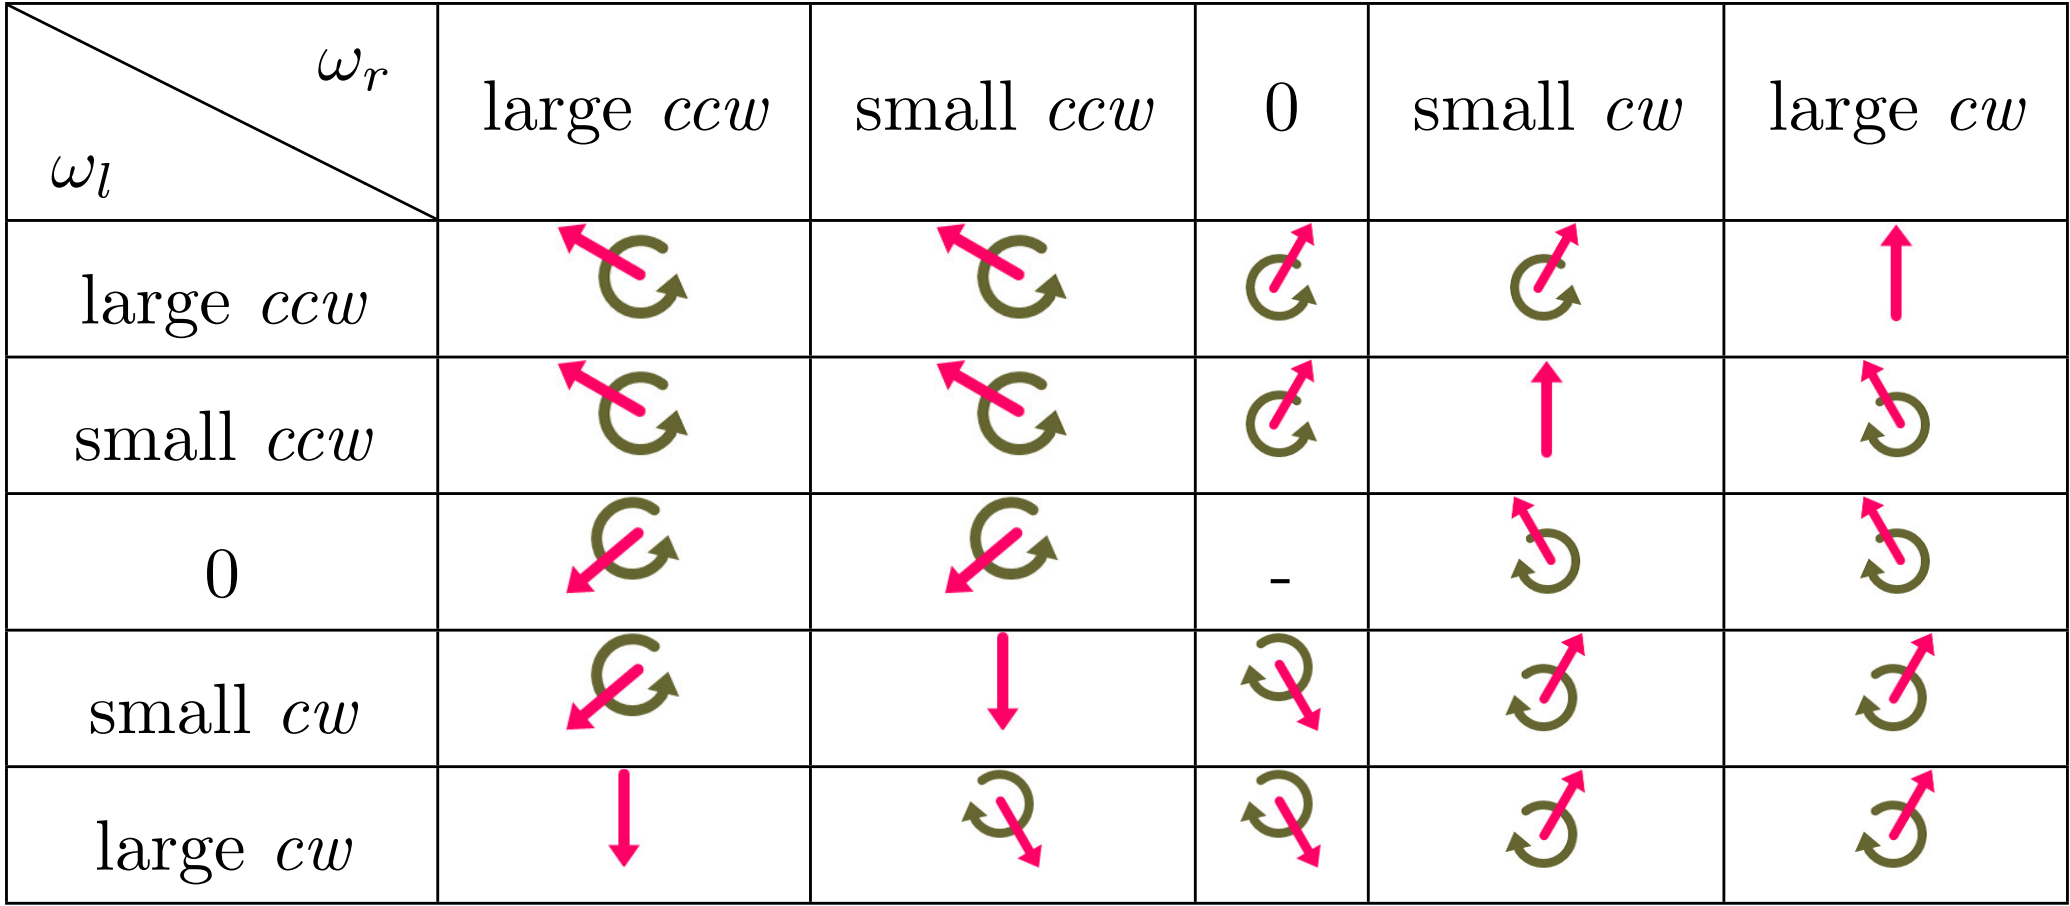
\includegraphics[width=1\columnwidth]{images/sd/screwdrive_maneuverability_nagaoka.png}
	\vspace{-10pt}
	\caption{Screwdrive Maneuverability \cite{Nagaoka2009a}}	
	%\vspace{-20pt}
	\label{fig:screwdrive_maneuverability}
\end{figure}


\begin{figure}[ht]
	\begin{subfigure}[t]{0.5\textwidth}
		\centering
		%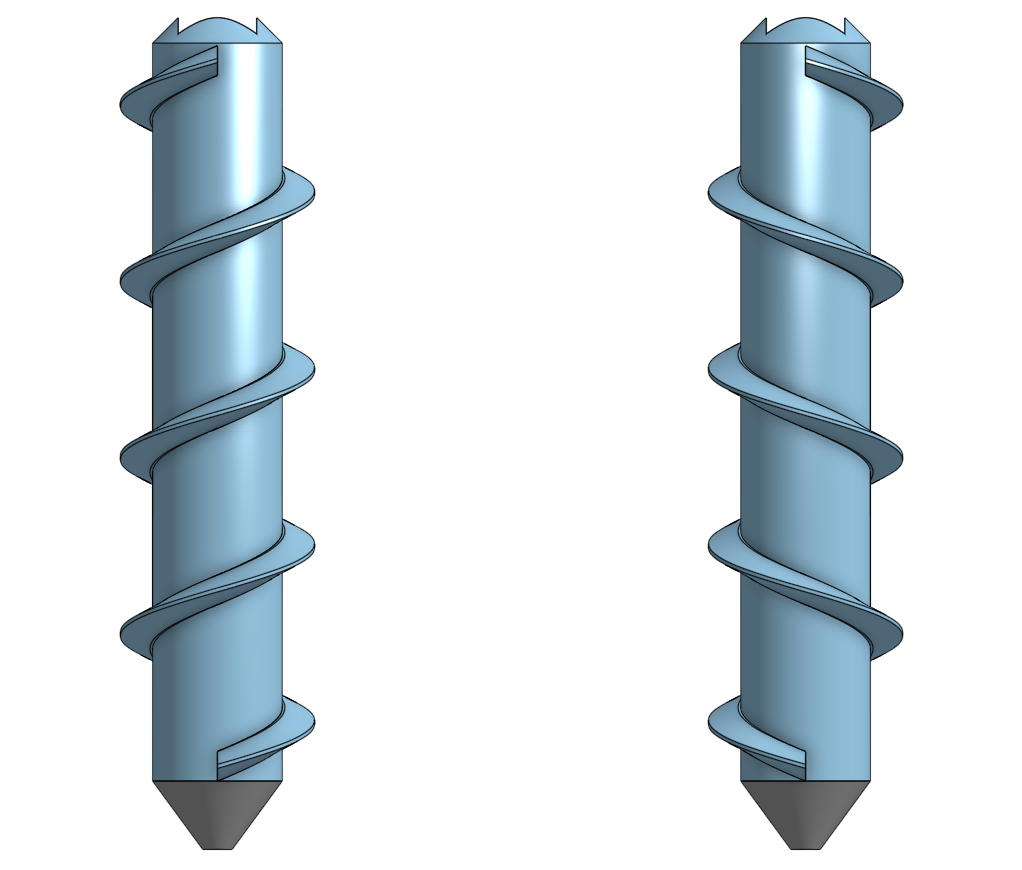
\includegraphics[width=1\columnwidth]{images/sd/screws_renders_dual_top.png}
		\includegraphics[width=1\columnwidth]{images/sd/screw_propulsion_FBD_alpha_0.pdf}
		\caption{Inter-screw angle of 0 degrees (parallel)}
		\label{fig:screw_FBD_alpha_0} 
	\end{subfigure}
	\begin{subfigure}[t]{0.5\textwidth}
		\centering
		%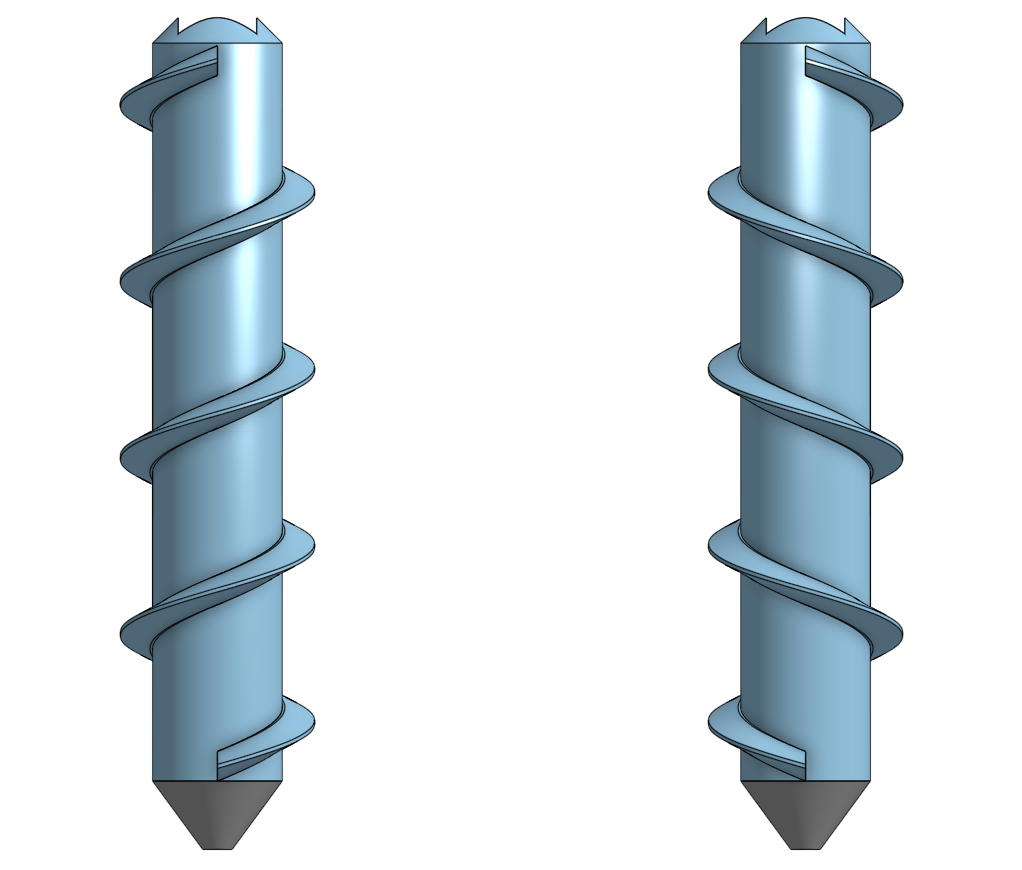
\includegraphics[width=1\columnwidth]{images/sd/screws_renders_dual_top.png}
		\includegraphics[width=1\columnwidth]{images/sd/FBD_two_screw_45_rigid_rotation.pdf}
		\caption{Inter-screw angle of 45 degrees}
		\label{fig:screw_FBD_alpha_45} 
	\end{subfigure}
	\caption{Screwdrive FBD Models}
	\label{fig:screwdrive_renders}
\end{figure}


%\begin{figure}[ht]
	%\begin{subfigure}[t]{0.5\textwidth}
		%\centering
		%\includegraphics[width=1\columnwidth]{images/sd/screw_propulsion_FBD_alpha_0.pdf}
		%\caption{Inter-screw angle of 0 degrees (parallel)}
		%\label{fig:screw_FBD_alpha_0} 
	%\end{subfigure}
	%\begin{subfigure}[t]{0.5\textwidth}
		%\centering
		%\includegraphics[width=1\columnwidth]{images/sd/screw_propulsion_FBD_alpha_45.pdf}
		%\caption{Inter-screw angle of 45 degrees}
		%\label{fig:screw_FBD_alpha_45} 
	%\end{subfigure}
	%\caption{TEST}
	%\label{fig:TESTS}
%\end{figure}



Research into screwdrive locomotion is centered, in large part, around its function in compliant media, such as soft terrains or fluids \cite{Dugoff1967, Cole1961, Nagaoka2011, Freeberg2010, Fales1972}, as this is where screwdrive systems excel. The degree of penetrability of the screw blade affects performance of the screws and consequentially a screwdriven vehicle. 

On rigid terrains where the blade cannot penetrate, the screwdrive behaves very differently both from a modeling and maneuverability perspective. Therefore, the screwdrive is dependent not only on the aforementioned geometric and functional parameters covered in section \ref{sec:screwdrive_parameters} but also on the properties of the medium it's in as well as the bearing load on the screws. 

% Force definition:
Screws provide a combination of tractive and rolling forces. \textbf{\emph{Rolling }} forces are those that result from oppositional frictional forces upon the body of the screw as it rotates, like a wheel, about its axis. These forces can be visualized as the forces that would be present were the screw blade not present, i.e. as if the screw was instead a roller. The addition of the screw blade adds \textbf{\emph{tractive}} forces. As the screw rotates, the blade displaces and moves along the medium adjacent to the blade surface creating longitudinal and lateral components of tractive force. The balance between the lateral and longitudinal components of the tractive force is highly dependent on the \emph{pitch angle}.

% TODO: add figure with force vectors 
Description of rolling and tractive forces depend on complex terramechanics models \cite{Nagaoka2010a, Cole1961}, fortunately, a more simple approach to these forces can be taken in order to determine the maneuverability of a screwdriven vehicle. Freeberg \cite{Freeberg2010} and Nagaoka et al. \cite{Nagaoka2009b} treat the rolling force similarly, while differing on their treatment of the tractive force. Nagaoka assumes the tractive force direction as perpendicular to the screw blade face, hence dependent on the \textbf{\emph{pitch angle}} and decomposable into longitudinal and lateral components, whereas Freeberg keeps only the longitudinal component of the tractive force. The combination of these \textbf{\emph{tractive}} and \textbf{\emph{rolling}} forces determine the resulting motion of the vehicle. 

Maneuverability is controlled by the ability of the screw to penetrate the medium, the relative orientation of the screws with respect to one another, and the screws' placement with respect to the vehicle body. When the screw penetrates the terrain, it has been found that the tractive forces dominate the rolling forces, the opposite has been found on rigid terrains. One exception found by Nagaoka \cite{Nagaoka2009a} is the case where the screws are rotating at a very slow speed in a penetrable terrain, under these conditions, the tractive forces do not outright dominate the rolling forces and some unwanted sideways motion is observed. Another exception has been documented \cite{Cole1961} when transitioning from water to land, when the vehicle will lurch as the screw initially rolls on the ground. 
%In Figure~\ref{fig:screw_FBD_alpha_0} two contra-rotating screws are shown.

The motions of a dual-screwdrive system in a penetrable terrain are shown in Figure ~\ref{fig:screwdrive_maneuverability}. These are shown from Nagaoka et al. \cite{Nagaoka2009a}, however, Freeberg's \cite{Freeberg2010} research is also in accordance. These motions arise from the combination of one of three actions possible through each of the two motors: clockwise, counterclockwise, or no rotational velocity. 

Since the screws are oppositely handed, longitudinal locomotion is achieved through contra-rotation of the screws at the same speed. This results in forward or backwards motion depending on the combination of the handedness of the screws and direction of screw rotation. 

The next case, skid turning, is that when one of the screws rotates and the other does not. Skid-turning results in a desirable tight-radius turn, however, it is terrain dependent and there are some situations where skid turning may not be optimum. Freeberg and Cole et al. have found that under low friction and low cohesion aground conditions, such as loose sand, skid-turning can result in the screw burying itself. In higher friction or highly cohesive terrains, such as clay, skid turning may not be possible as this requires more force.  

Finally, when both screws turn in the same direction there are two motions possible dependent, once again, on terrain. In water, this leads to a rotation of the vehicle with no net traversal motion, this is known as point-turning. Aground, it leads to arc turning of various radii, depending on the type of terrain. Freeberg \cite{Freeberg2010}, found that clay, gravel, loose sand, and dirt produced wide arcs, whereas grass and marshlands procuded smaller-radius arc. The commonality being that these motions involved a rotation of the vehicle as well as a net displacement. 

Nagaoka et al. \cite{Nagaoka2009a} also explored the case where both screws were actuated but at different directions and speeds, producing arc turning, which they refer to as steering. This steering is useful as it would permit adjustments to heading while the robot is in motion. 





%\subsubsection{Variable Pitch Screws}
%\label{sec:screwdrive_variable_pitch}

\subsubsection{Variable Geometry Screws Origami}
\label{sec:screwdrive_variable_pitch}

\begin{figure}[htb]
    \begin{subfigure}{0.5\textwidth}
    \centering
    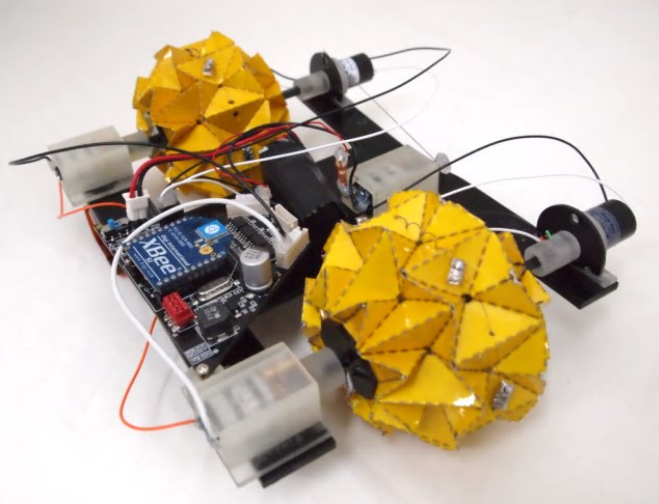
\includegraphics[width=.90\columnwidth]{images/origami_lee2013.png}
    \caption{Deformable wheel robot, \cite{Lee2013}.}
    %\vspace{-20pt}
    \label{fig:origami_lee}
    \end{subfigure}
    \begin{subfigure}{0.5\textwidth}
    \centering
    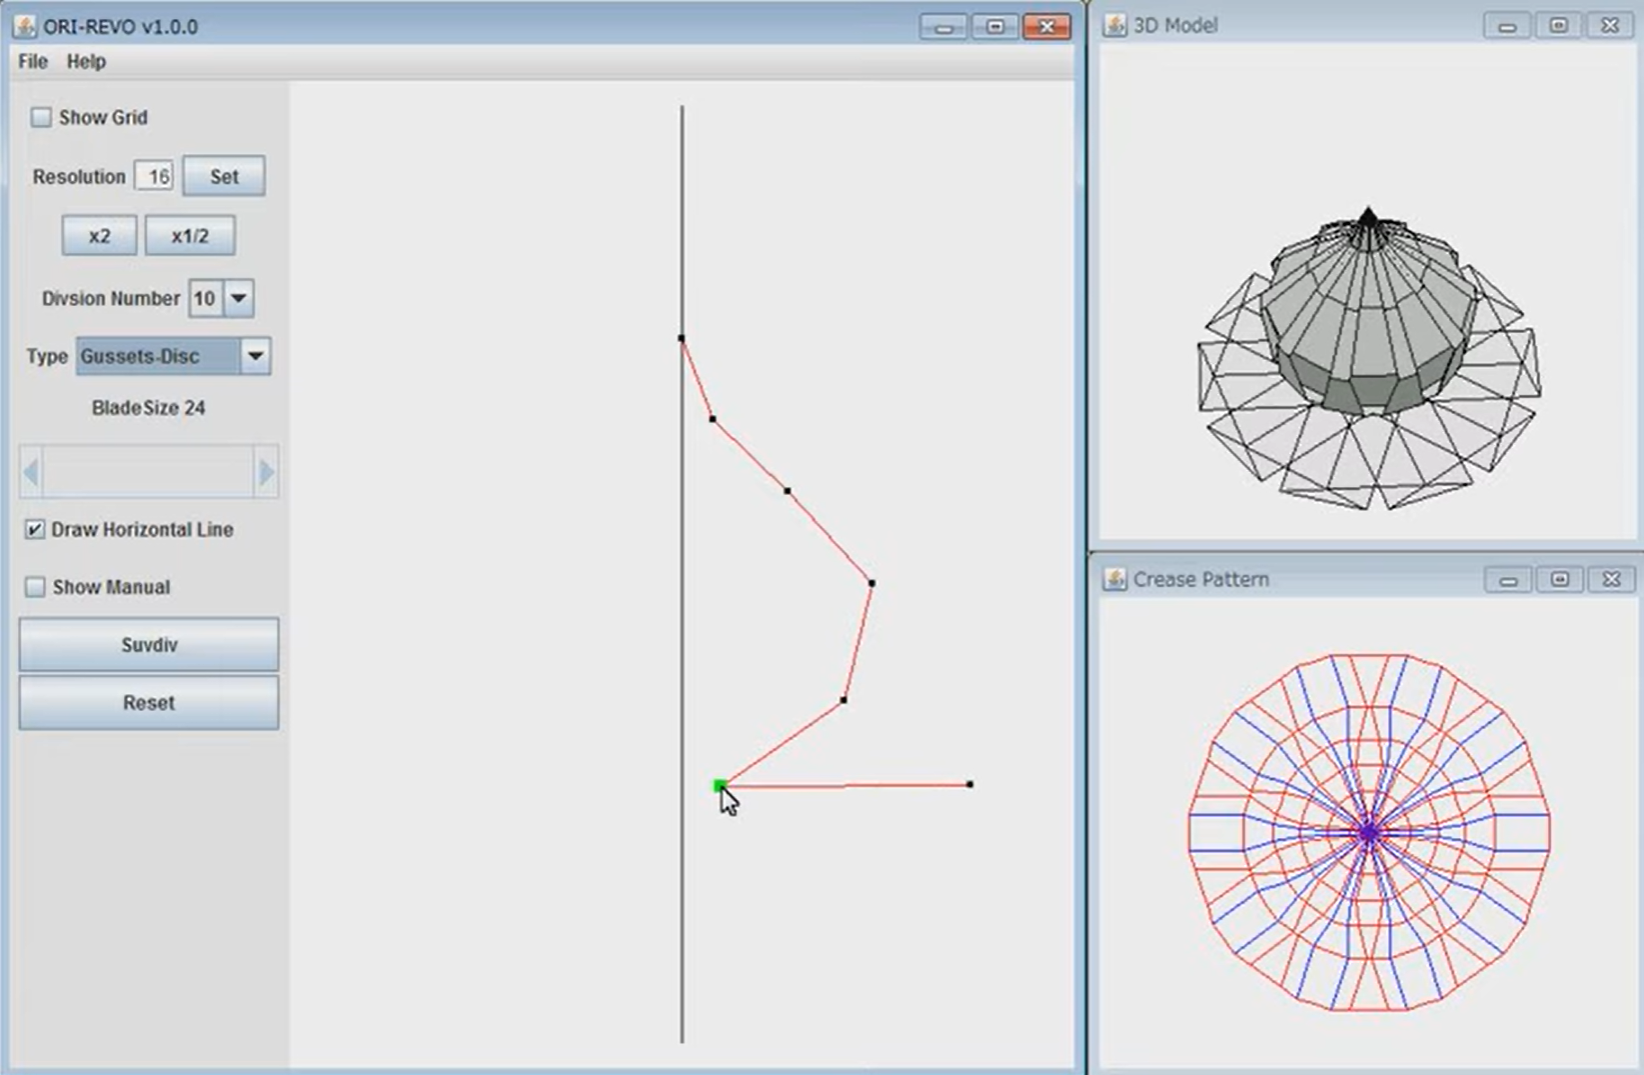
\includegraphics[width=1.10\columnwidth]{images/origami_orirevo.png}
    \caption{ORI-REVO software, \cite{Mitani2009}.}
    %\vspace{-20pt}
    \label{fig:origami_orirevo}
    \end{subfigure}
    \caption{Origami applications and software}
    \label{fig:origami_lee_orirevo}
\end{figure}

%\begin{figure}[!htb]
    %\centering
    %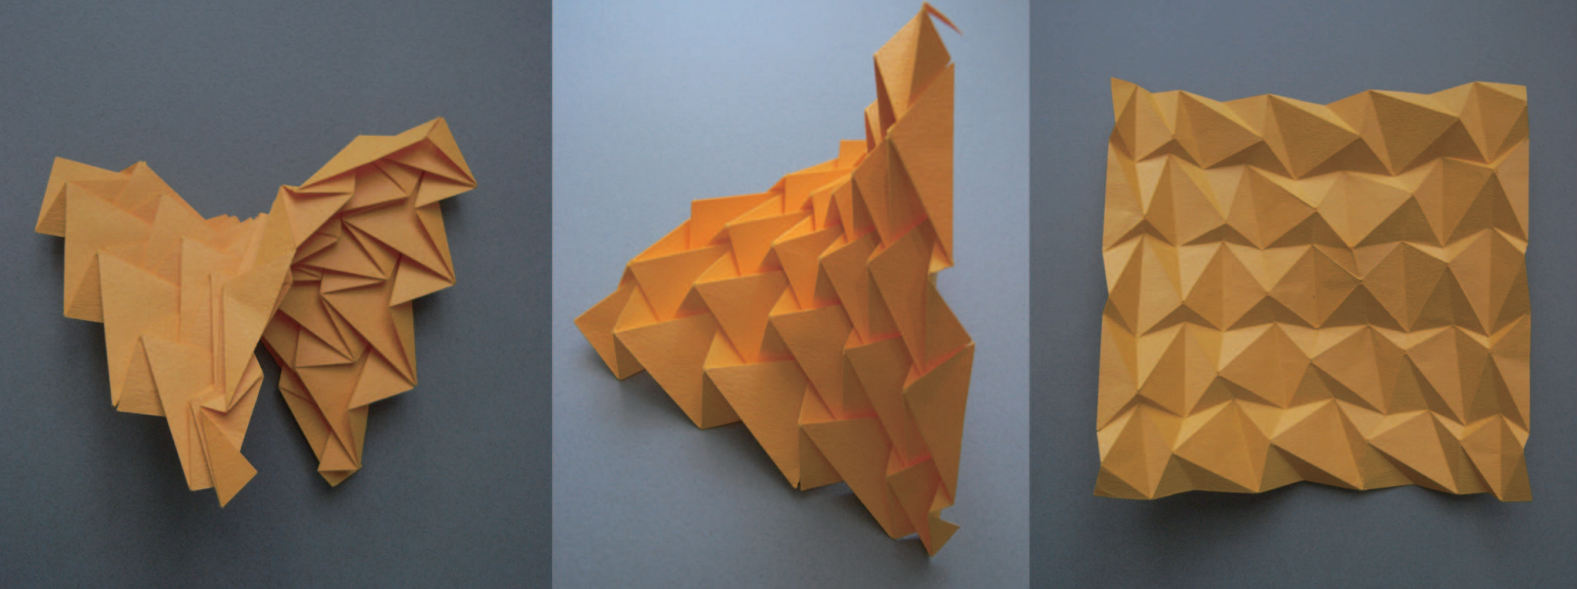
\includegraphics[width=.90\columnwidth]{images/origami_tachi2010_complex_real.png}
    %\caption{Origami structures, \cite{Tachi2010}.}
    %\vspace{-20pt}
    %\label{fig:origami_tachi_complex_real}
%\end{figure}


%Motivation
Once optimal screw parameters for a given set of terrains are found and an onboard terrain classification system provides the type of terrain, a variable pitch screw would allow switching between different sets of geometries to best suit the terrain. 

Origami is an art form that is increasingly being looked to for its ability to create folding structures from a two dimensional pattern, from MEMS devices \cite{yan2016}, to robotic crawling actuators \cite{Rafsanjani2018}, to deformable wheels \cite{Lee2013}, and medical microrobots \cite{Miyashita2015} this technique allows creation of metamaterials that can be actuated with a single degree of freedom. In metamaterials, the resulting structure depends not only on the underlying construction material, but also the geometry, leading to structures that can exhibit wildly different properties, such as stiffness, compressive moduli, etc, than their base material. 

Current fabrication methods for the screws utilize three dimensional printing. While useful for initial prototypes, utilizing a laser cutter would decrease fabrication time significantly as Silverberg et al. \cite{Silverberg2015} and Rafsanjani \cite{Rafsanjani2018} have found. Furthermore, this fabrication method could provide the means by which to design and fabricate a robust variable pitch screw with a high degree of robustness as compared to an articulated variable pitch device. 

%Furthermore, generating origami via traditional hand-folding methods, while simple, creates pre-creases in the material that are not necessary in the final structure but are nevertheless present and affect stiffness, adding additional degrees of freedom to the structure. 

%In \cite{Silverberg2014a} Silverberg utilized dash-and-gap perforations since it was found that continuous line patterns lead to lattices that are easy to tear and exhibit anisotropic bending properties. Dash-and-gap, on the other hand, allowed isotropic bending properties and equal folding stiffness for valley and mountain creases. Another form of manufacture would be a two step process where the laser would make engravings of mountain or valley folds instead of cutting all the way through. This would lead to a stronger and sealed surface which is desirable ingress protection. 

Lee et al.\cite{Lee2013} create an active origami wheel using the waterbomb, or magic ball, origami pattern for the structure and a combination of passive elements, such as a spring, and smart wire actuators to achieve changes in its shape, Figure ~\ref{fig:origami_lee}. Silverberg et al. \cite{Silverberg2015} utilize the Miura-ori tesselated folding pattern to create structures comprised of individual cells that are bistable, that is they settle into decreased energy minima. This switchable behavior would be pertinent in actuator design as it would allow structures that have two stable passive states with energy needed only to switch states. 

%The magic ball pattern is comprised of individual unit structures, in this case triangles, that exhibit independent behavior but can be chained to produce a bulk structure composed of individual switchable units, as in Figure ~\ref{fig:origami_lee}. 


%Furthermore, they showed that many structures can arise from the same underlying patterns by localized push-through-defects. One could imagine a robot hull made of a Miura-ori tesselated surface where each unit cell is actuated via an individual actuator to change the outer structure of the robot in real-time. 

%\begin{figure}[!htb]
    %\centering
    %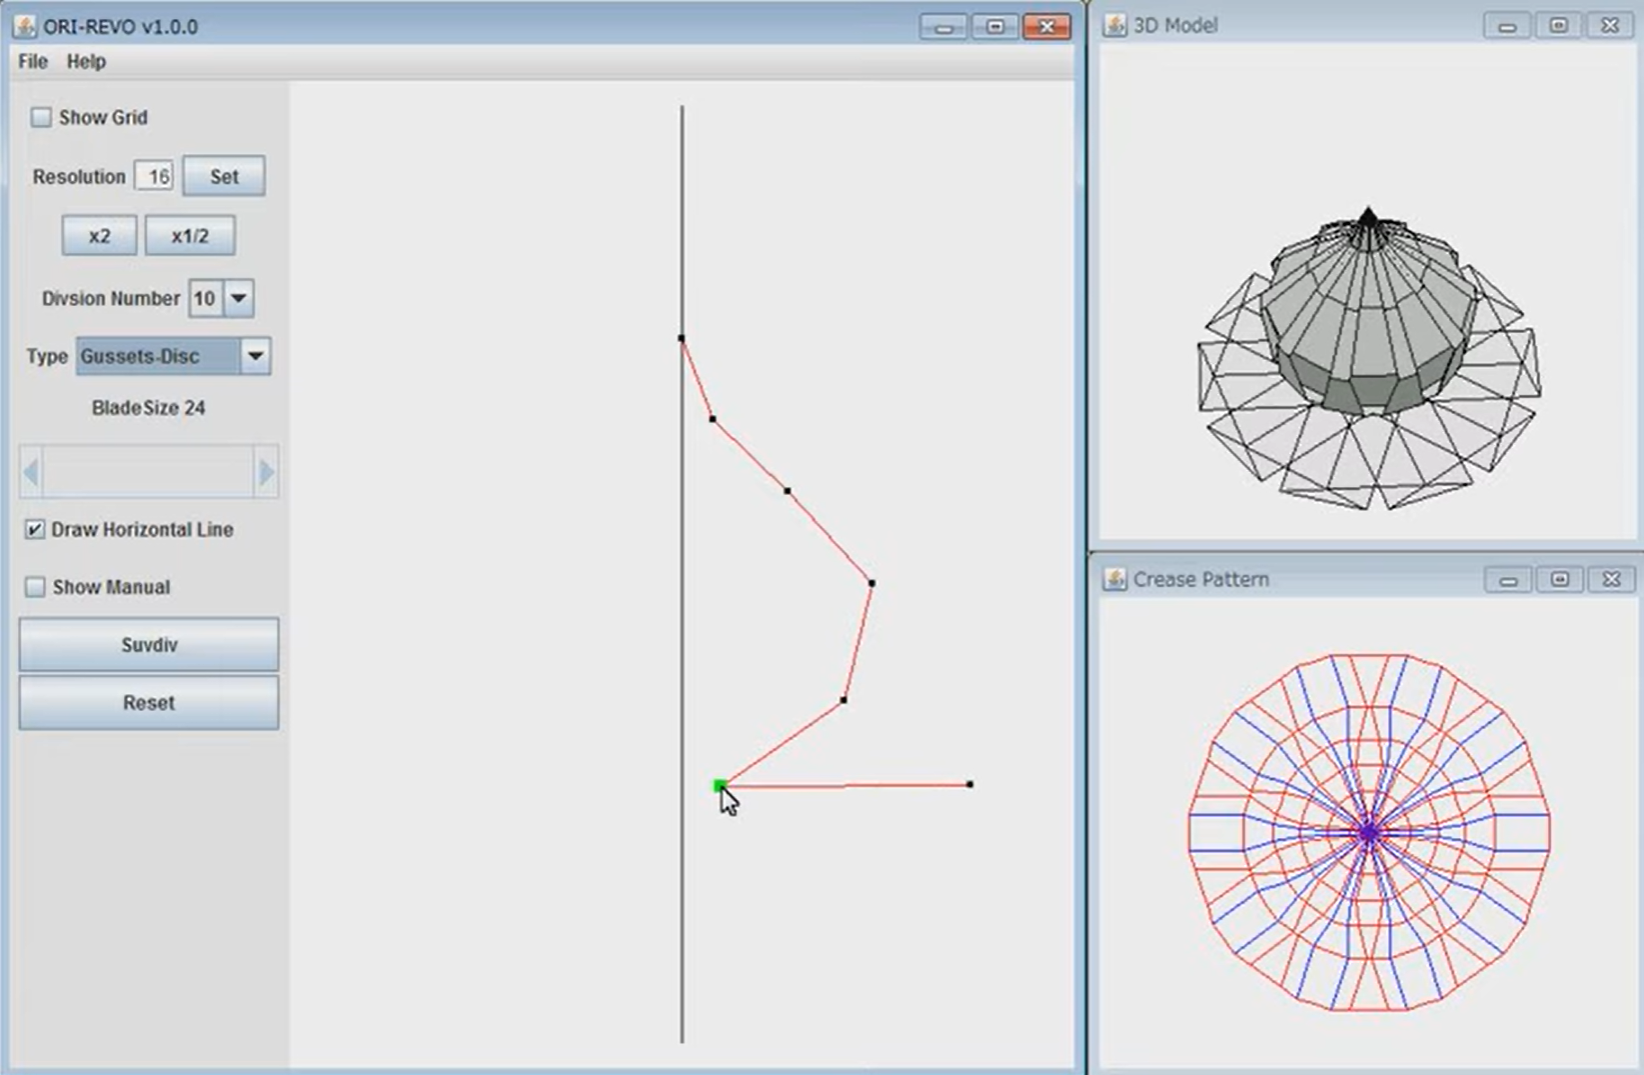
\includegraphics[width=.90\columnwidth]{images/origami_orirevo.png}
    %\caption{ORI-REVO software, \cite{Mitani2009}.}
    %\vspace{-20pt}
    %\label{fig:origami_orirevo}
%\end{figure}



With this project, we propose development of a screw using origami principles to achieve an actuatable surface capable of transitioning between two distinct stable configurations and where the limits are set either mechanically or by exploiting origami bistability. 

% inverse design problem 
In order to do this a crease pattern needs to be generated to create the target design, this is known as the inverse design problem. Castle et al. \cite{Castle2014} programatically tackle the inverse problem of designing cuts and folds in a 2D surface to obtain a given 3D object. The justification of the cuts is that there are features that can be obtained more effectively by removing material.  


Boyle et al. created a complex double curvature three dimensionaly face from an initially flat 3D-printed surface. This is known as shape-morphing or active origami principles, there the morphing occurs due to an external stimuli, such as pneumatics or, in this case, temperature differences. 3D inverse design was used to specify the target shape and then work backwards to program the metamaterial. 	

Mitani et al. \cite{Mitani2009} created the ORI-REVO software which allows creation of revolution surfaces by specifying a profile pattern, see Figure ~\ref{fig:origami_orirevo}. This tool also allows the specification of division number, resolution, as well as manual manipulation in real time. The resultant 3D form is shown in the top right and the crease pattern in the bottom right. %rotational symmetry


Morever actuation forces need to be computed in order to specify the actuator. Fuchi et al. \cite{Fuchi2013} have developed OMTO (an origami modeling toolbox for matlab) which uses FEM to set boundary conditions, fixed points, and forced point to calculate fold lines that optimize greatest displacement in specified directions at the output nodes. In 2018, Gillman \cite{Gillman2018} continued this work adding nonlinear optimization yet removing the graphical user interface. 





%\begin{figure}[htb]
    %\centering
    %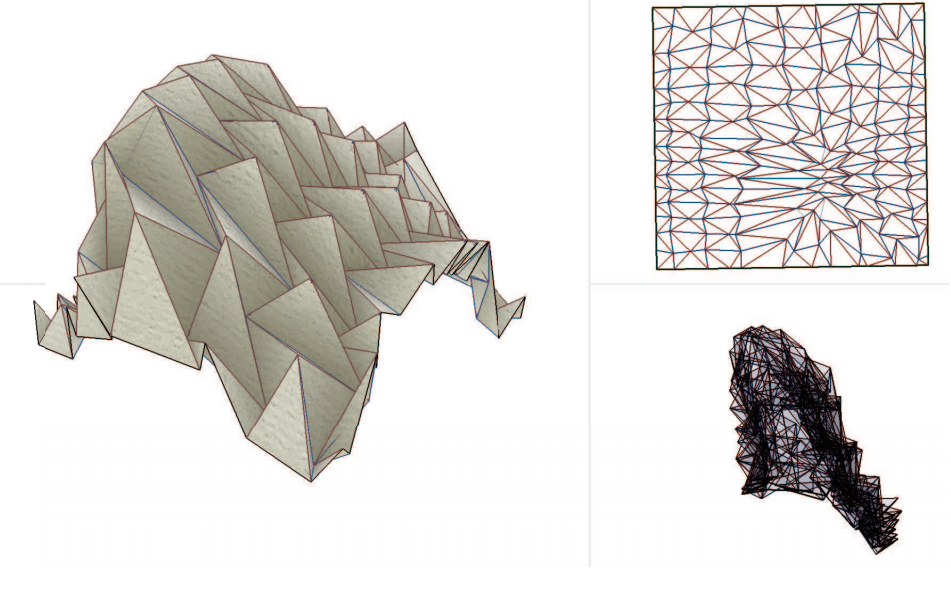
\includegraphics[width=.90\columnwidth]{images/origami_tachi2010_complex_pattern.png}
    %\caption{Complex origami forms, \cite{Tachi2010}.}
    %\vspace{-20pt}
    %\label{fig:origami_tachi_complex_pattern}
%\end{figure}









%%% MERGE ABOVE AND BELOW


%\begin{figure}[htb]
    %\centering
    %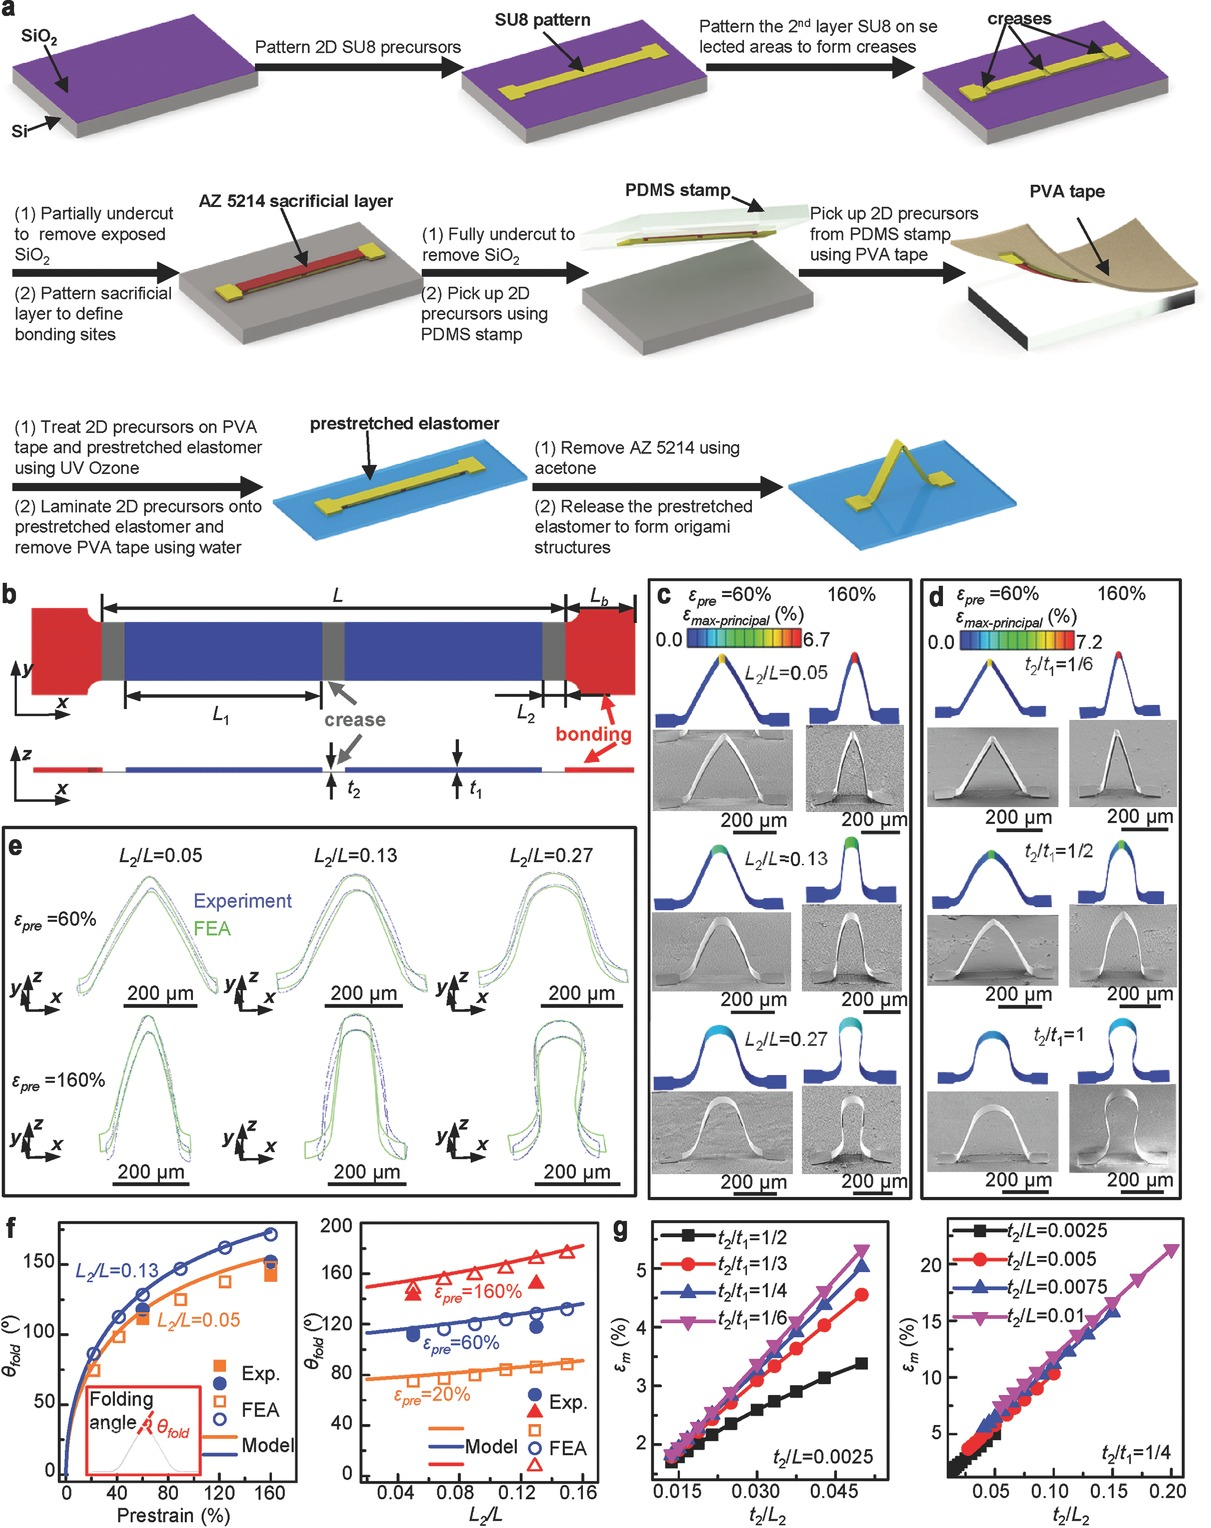
\includegraphics[width=.90\columnwidth]{images/lit_review/yan2016_origami_mems_folds.jpg}
    %\caption{Controlled Mechanical Buckling for Origami‐Inspired Construction of 3D Microstructures in Advanced Materials, \cite{yan2016}.}
    %\vspace{-20pt}
    %\label{fig:origami_mems}
%\end{figure}

%\begin{figure}[htb]
    %\centering
    %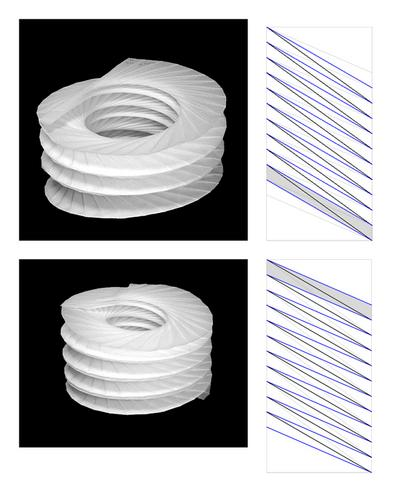
\includegraphics[width=.90\columnwidth]{images/lit_review/azuma_origami_convolution.jpg}
    %\caption{Azumi et al.'s convolutional helix, \cite{yan2016}.}
    %\vspace{-20pt}
    %\label{fig:origami_mems}
%\end{figure}


%computational origami https://langorigami.com/article/computational-origami/ 

%\emph{Programmability of the lattice expansion}
%Programmability of the lattice expansion to redirect force exerted by screws on land due to a morphed geometry. This programmability has been demonstrated by Rafsanjani et al \cite{Rafsanjani2018} in which they programmed their actuator's expansion as is required to achieve a snake like crawl, in which some scales contract while others expand, leading to overall positive net displacement. 
%
%Photo of snake actuator. 
%Bistability
%Methods
%Laser cut of valley and mountain folds
%Image of laser cut delrin
%Itae Cohen's supplemental material? 
%%Algorithms?laser


%Software: ORI-REVO
%" This software is a design software that allows users to interact with origami forms while altering the crease pattern of the model. The software can keep: Developability (foldable from a piece of paper) Flat-foldability (foldable into a flat shape) Planarity of facets (paper do not twist in 3D form) Point coordinate coincidence Paper size "

% WATERBOMB FIGURE
%\begin{figure}[htb]
    %\centering
    %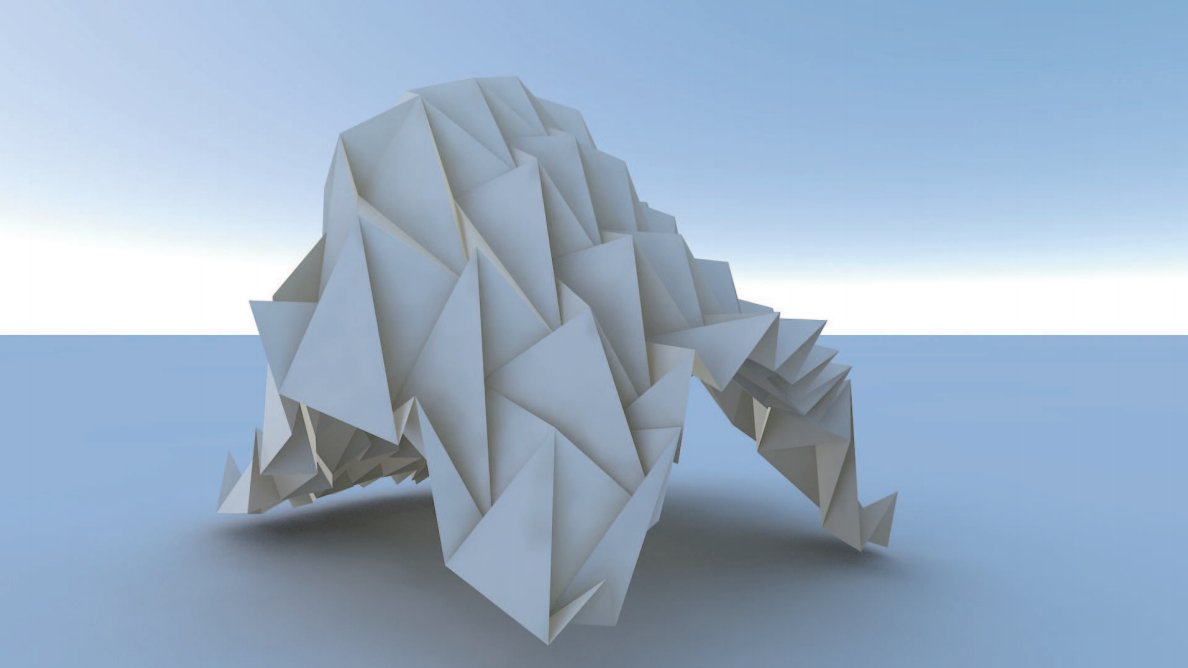
\includegraphics[width=.90\columnwidth]{images/origami_tachi2010_complex.png}
    %\caption{Waterbomb origami forms, \cite{Tachi2010}.}
    %\vspace{-20pt}
    %\label{fig:origami_tachi_complex}
%\end{figure}






%The combination of these forces determines the resulting motion of the vehicle. While Cole \cite{Cole1961} and those involved in the MSA and RUC studied the parameters of the vehicles in detail, Freeberg and Nagaoka classified the maneuverability of screwdriven systems. 




%Turning 
%Skid-turning 
%Arc-turning 
%Pivot-turning 

%NAGAOKA info
%Abstract deliveration the hypothetical usage of a double screw design for moon rover propulsion for its ability to navigate "regolith", the fine soil terrain found on the moon. Skid steering is another benefit of this propulsion type as it does not require an additional steering mechanism but it can instead be accomplished by a differential in screw speed. \cite{Nagaoka2011}
%Nagaoka et al. \cite{Nagaoka2011} make a prototype design using screw propulsion called the Screw Drive Robot and a simplified dynamic model for movement on loose soil is presented. 
%When surmounting small obstacles, forward locomotion was not successful, however, lateral movement climbing of small rocks. This is hypothesized to be due to the rolling motion, as would have a standard wheel. As a wheeled-robot it was capable of climbing a rock about half of the screw's diameter. % #maneuverability 



%\subsubsection{Screwdrive configurations}
%Freeberg \cite{Freeberg2010} studied the use of alternatives to the dual-screw configuations, venturing into three and four screw arrangements. 

%The quad-screw configurations consisted of four screws arranged in three different geometric layouts. The first, \emph{split screw}, used a pair of screws aligned in parallel and with the same blade handedness on each side, as if it were a dual screw configuration with the screws split in half, hence the name. Changing the handedness of either the two front or back screws produced the \emph{inline-screw}. The \emph{cross-screw} configuration took the inline-screw and rotated all four screws 45 degrees to create an "x" pattern. Finally, the \emph{diamond} configuration rotated the inline-screw screws towards the outside, creating a diamond configuration.

%Freeberg found that split screw performed in much the same way as the dual screw on soft terrain, however, it could also rotate about its center. 

%The inline-screw configuration was found to be the most promising as it also allowed rotation about the center but also more controlled lateral motion than the split-screw. The result being controllable and reversible longitudinal, lateral, and rotational motions. 

%The diamond and cross configurations were found to have similar characteristics as the inline-screw but with indeterminate longitudinal and lateral motions, respectively. This is due to the interplay of tractive and rolling forces for the parameters chosen. 


\subsubsection{Proposed Research}

%The proposed research section (or sections) is the key element of the proposal and should comprise no less than half the page limit set for the project description. This section should outline the plan of work, including the activities to be undertaken, and a description of experimental and/or computational methods and procedures. It should address what will be done, how it will achieve the proposed objectives, and should contain justification for the approach proposed. The proposed research section should complete the arguments developed earlier and present initial ideas on how to solve the problems posed. Strong proposals avoid repetition and digression. This section (or sections) should relate the proposed activities to the project objectives and provide expected outcomes, including how the proposed research, if successful, will contribute to a greater understanding of the topical area. An assessment of risk should be provided with the proposed research as well as a contingency plan in case a particular research avenue proves inexpedient in some manner. It should present a reasoned path from where the student begins to where they want to be at the end of the research.


Screwdrive locomotion is feasible and desireable as a simple, robust, and inexpensive form of amphibious locomotion. As with any novel method of locomotion, more research is needed to appropriately describe its nuanced aspects. In particular, it has been shown that while screwdrive locomotion works well aground and afloat, its maneuverability, motion model, and design parameters differ for both limit scenarios. Moreover, within aground performance, parameter and locomotion strategies can change not only based on the type of terrain (snow, sand, dirt) but also on time-dependent conditions, such as friction and cohesion, which are dependent on the level of moisture in the ground.

Given the variable nature of the terrain and types of terrain a screwdrive vehicle is capable of navigating, developing a dynamic model that learns its parameters in real-time would be advantageous and responsive. This online model would also allow detection of transition between different terrains, in particular aground and afloat conditions, and react accordingly. This model would build on the efforts of \cite{Rogers-Marcovitz2014} et. al, who used an Extended Kalman Filter to identify changing parameters of the models based off predicted trajectories and sensed trajectories. This work was done to correct for slip, however it should also be applicable to the screwdrive. 


Given correct characterization of the system for known terrain types, it would be possible to identify characteristics about the terrain based on deviations from expected motions. Giguere et. al \cite{Giguere2010} designed an unsupervised system capable of classifying different types of terrain, such as grass, sand, and linoleum, using an onboard IMU and actuator feedback. We propose to build a simpler system that will allow detection between water and land, as well as the intermix region in order to change screw parameters. 

Lastly, we propose utilizing origami to create variable morphology screws that can be used to alternate between approximate optimal parameters for the water and land use cases. This effort will require the modeling, design, and implementation of screws in such a way that the actuation can occur online and in a way that is feasible on a robot of this size and complexity. 

\begin{itemize}
	\item Characterization optimal screw parameters for land/water locomotion.
	\item Development of a dynamic model for a number of terrains including land and water.
  \item Development of terrain classification algorithms utilizing onboard IMU and actuator feedback. 
  \item Development of a variable morphology screw actuator. 
	\item Integration of all of the above in order to achieve a system that properly classifies its environment and adapts its actuators' characteristics to match it. 
\end{itemize}

%\[ m_v \ddot{X}_m = \sum\limits_{i=1}^{\overline{N}} \Big( sgn(\omega_r)(f_r - F_{ri}sin\eta_r) +   sgn(\omega_l)(f_l - F_{li}sin\eta_l) \Big) - C_X R_X \]

%\[ m_v \ddot{Y}_m = \sum\limits_{i=1}^{\overline{N}} \Big( sgn(\omega_r) F_{ri} cos(\eta_r) -   sgn(\omega_l) F_{li}cos(\eta_l) \Big) - C_Y R_Y \]

%\[ I_r \ddot{\delta} = \sum\limits_{i=1}^{\overline{N}} \Big( sgn(\omega_r) F_{ri} r_{ri} cos(\eta_r - b_{ri}) +   sgn(\omega_l) F_{li}r_{li}cos(\eta_l - b_{li}) \Big) - C_\delta R_\delta L_W \]

%where, 

%\[ 
%\left \{
  %\begin{tabular}{ccc}
  %\( \eta_r = \eta_l = \eta \) & : \(\eta = const. \)  \\
  %\( b_{ji} = arctan(\frac{L_{ji}}{L_W}) \) & : j= r,l  \\
  %\( r_{ji} = \sqrt{L^2_{ji} + L^2_W} \) & : j= r,l  \\
  %\( L_{ji} = \lvert \frac{L}{2} - (i-1)p - p sin \theta_j \rvert \) & : j= r,l   
  %\end{tabular}
%\right.
%\]

%\[ m_r X_m = sgn(\omega_r) \]




%%
%Propulsive force, skin friction, and soil shear models are studied in \cite{Nagaoka2009b}. Soil shear model was found to be more statistically suitable than the skin friction model suggesting propulsion of the screwdrive being more dependent on shear than skin friction.

%Nagaoka et al. \cite{Nagaoka2011} present two models: one based on skin friction and soil shear, the other based on terramechanics. The skin friction can be modeled simply with the terrain-screw friction coefficients and the screw geometry and allows simulation of the locomotion trajectories. The terramechanics model is more suited towards modeling drawbar pull, and  both normal and shear stresses. A third model, called the interaction model, combines these two prior efforts to better model the forces and medium transport. 

%The interaction model combines skin friction and soil shear, models the behavior of both the screw and the soil caught in each screw flight, compaction and shear characteristics of the soil, and permits quantitative evaluation of the screw geometry's effect on tractive performance. 
%%


%Equations of motion given for the parallel dual-screw system in terms of velocity of the screws, screw angle, "coefficients of signal"? (did they mean friction?), the propulsive forces based off the barrel and screw flight, and frictional resistance in the x and y direction. 

%\textcolor{red}{Figure 4} shows the possible trajectories for cases where there is same speed, opposite direction, which results in net positive or backward, then same speed same direction, which results in a strafe left or right, and one screw spinning twice as fast as the other, resulting in diagonals which are dependent on the helix angle (60 in the case shown). Additionally, in the cases of diagonal motion, the yaw angle of the vehicle changes, rotating about as it translated diagonally. Presumably, a helix angle of 45, would result in non-yaw rotations. 

%This also suggest that non 45 degree angles can be used for yaw-control. The study also suggest that the screw angle is the most important parameter during the simulation, as well as any shaping effects that external forces might have. 

%They find that its a nonholonomic affine system and FR can be seen to be reaction against movement, thus attenuating the propulsive forces. 

%Simplified model is derived for Y double dot as  a function of a constant multiplied by x double dot. 
%\cite{Ellefsen2012} %drifting 
%\cite{Giguere2010}


